%{{{-----------------------------------Basics----------------------------------%

%document class definition
\documentclass[
    11pt,
    a4paper,
    oneside,
    headinlcude, footinclude,
    twoside,
]{report}


%essential packages
\renewcommand*\rmdefault{ppl}
\usepackage[top=2.5cm,bottom=2.5cm,left=3cm,right=3cm]{geometry}
\usepackage[english]{babel}
\usepackage[T1]{fontenc}
\usepackage[utf8]{inputenc}
\usepackage{xcolor}
\usepackage{amssymb}


%additional packages
\usepackage{amssymb}
\usepackage{amsmath}
\usepackage[framemethod=Tikz]{mdframed} % for the "important" boxes
\usepackage{tikz} % to draw figures
\usepackage{enumerate} % to customize the type of enumerate you want
\usepackage{pgf,tikz,pgfplots} % for the transfer from geogebra to tikz
\usepackage{mathrsfs}% for the transfer from geogebra to tikz
\usepackage{graphicx} % to include pictures
\usepackage{stackrel}
\usepackage{fancyhdr}
\usepackage{tabularx}
\usepackage{makecell} % to make thick hlines in the front page
\usepackage[makeroom]{cancel}
%}}}

%{{{-----------------------------------Macros----------------------------------%

\newcommand{\myImplies}[0]{\rightarrow}

\newcommand{\powerset}[1]{\mathcal{P}(#1)}

\newcommand{\tvect}[3]{%
   \ensuremath{\Bigl(\begin{smallmatrix}#1\\#2\\#3\end{smallmatrix}\Bigr)}}

\newcommand{\myVector}[3]{\begin{pmatrix}#1\\#2\\#3\end{pmatrix}}

\newcommand{\tq}[0]{\textrm{t.q.}}

\newcommand{\markDate}[1]{\begin{flushright}#1\end{flushright}}

\newcommand{\cqfd}[0]{\begin{flushright}$\Box$\end{flushright}}

\renewcommand{\vec}[1]{\overrightarrow{#1}}

\def\getangle(#1)(#2)#3{
    \begingroup
        \pgftransformreset
        \pgfmathanglebetweenpoints{\pgfpointanchor{#1}{center}}{\pgfpointanchor{#2}{center}}
        \expandafter\xdef\csname angle#3\endcsname{\pgfmathresult}
    \endgroup
}

\newcommand\Warning{
    \makebox[1.4em][c]{
    \makebox[-5.5pt][c]{\raisebox{.2em}{!}}
    \makebox[0pt][c]{\color{red}\huge$\bigtriangleup$}}
}

%colored frame box
\newcommand{\cfbox}[2]{
    \colorlet{currentcolor}{.}
    {\color{#1}
    \fbox{\color{currentcolor}#2}}
}

%}}}

%{{{----------------------------------Settings---------------------------------%

\title{Physics}

\author{Arnò Fauconnet}

\setlength{\parindent}{0pt} %disable initial indent on first paragraph of sections in the whole doc

% the style of the boxes
\newmdenv[
        roundcorner=10pt,
        middlelinecolor=red,
        backgroundcolor=gray!15,
        linewidth=2pt,
        frametitlerule=true]{highlightBox}

% increases the space between paragraphs
\setlength{\parskip}{.3em}

\usetikzlibrary{calc}
\usetikzlibrary{arrows}%for the transfer from geogebra to tikz
\pgfplotsset{compat=1.15}


% Geogebras wierd colors xD
\definecolor{ffffff}{rgb}{1.,1.,1.}
\definecolor{qqqqff}{rgb}{0.,0.,1.}
\definecolor{qqffqq}{rgb}{0.,1.,0.}
\definecolor{ffqqtt}{rgb}{1.,0.,0.2}
\definecolor{ududff}{rgb}{0.30196078431372547,0.30196078431372547,1.} 
\definecolor{ffqqqq}{rgb}{1.,0.,0.} 
\definecolor{xdxdff}{rgb}{0.49019607843137253,0.49019607843137253,1.}
\definecolor{zzttqq}{rgb}{0.6,0.2,0.}
\definecolor{uuuuuu}{rgb}{0.26666666666666666,0.26666666666666666,0.26666666666666666}
\definecolor{wwccff}{rgb}{0.4,0.8,1.}
\definecolor{qqttcc}{rgb}{0.,0.2,0.8}
\definecolor{ffwwzz}{rgb}{1.,0.4,0.6}
\definecolor{ttqqqq}{rgb}{0.2,0.,0.}
\definecolor{qqccqq}{rgb}{0.,0.8,0.}
\definecolor{ffwwqq}{rgb}{1.,0.4,0.}
\definecolor{xfqqff}{rgb}{0.4980392156862745,0.,1.}
\definecolor{wwqqcc}{rgb}{0.4,0.,0.8}

\tikzstyle{every node}=[font=\large]

\graphicspath{ {Physics/figures/} }


% header and footer settings
\pagestyle{fancy}
\fancyhf{}
\fancyhead[LE,LO]{Arnaud Fauconnet}
\fancyhead[CE,CO]{\textsc{Physique}}
\fancyhead[RE,RO]{MAN - Printemps 2019}
\fancyfoot[CE,CO]{\leftmark}
\fancyfoot[LE,RO]{\thepage}

\renewcommand{\headrulewidth}{2pt}
\renewcommand{\footrulewidth}{1pt}
%}}}

%%%%%%%%%%%%%%%%%%%%%%%%%%%%%%%%%%%%%%%%%%%%%%%%%%%%%%%%%%%%%%%%%%%%%%%%%%%%%%
%----------------------------------------------------------------------------%
%-------------------------------Text starts here-----------------------------%
%----------------------------------------------------------------------------%
%%%%%%%%%%%%%%%%%%%%%%%%%%%%%%%%%%%%%%%%%%%%%%%%%%%%%%%%%%%%%%%%%%%%%%%%%%%%%%


\begin{document}

\begin{titlepage}
   \begin{center}
       \vspace*{\fill}

       {\Huge EPFL}\\ 
%----------------------------------------------------------------------------%
       \vfill
       {\huge MAN}\\ [1em]
       {\Large Mise à niveau}\\
%----------------------------------------------------------------------------%
        \vfill
        \begin{tabularx}{\textwidth}{X}
            \Xhline{3\arrayrulewidth}\\
        \end{tabularx}\\ [2em]
        {\Huge Physique} \\ [1em]
        \textsc{\huge Prepa-033} \\ [2em]
        \begin{tabularx}{\textwidth}{X}
            \Xhline{3\arrayrulewidth}\\
        \end{tabularx}\\ [2em]
%----------------------------------------------------------------------------%
        \vspace{.7cm}
        {\large
        \begin{tabularx}{.9\textwidth}{Xr}
            \textit{Student:} & \textit{Professor:}\\
            Arnaud \textsc{Fauconnet} & Sylvain \textsc{Bréchet}
        \end{tabularx}}
%----------------------------------------------------------------------------%
        \vfill
        {\Large Printemps - 2019}

%----------------------------------------------------------------------------%
        \vfill
        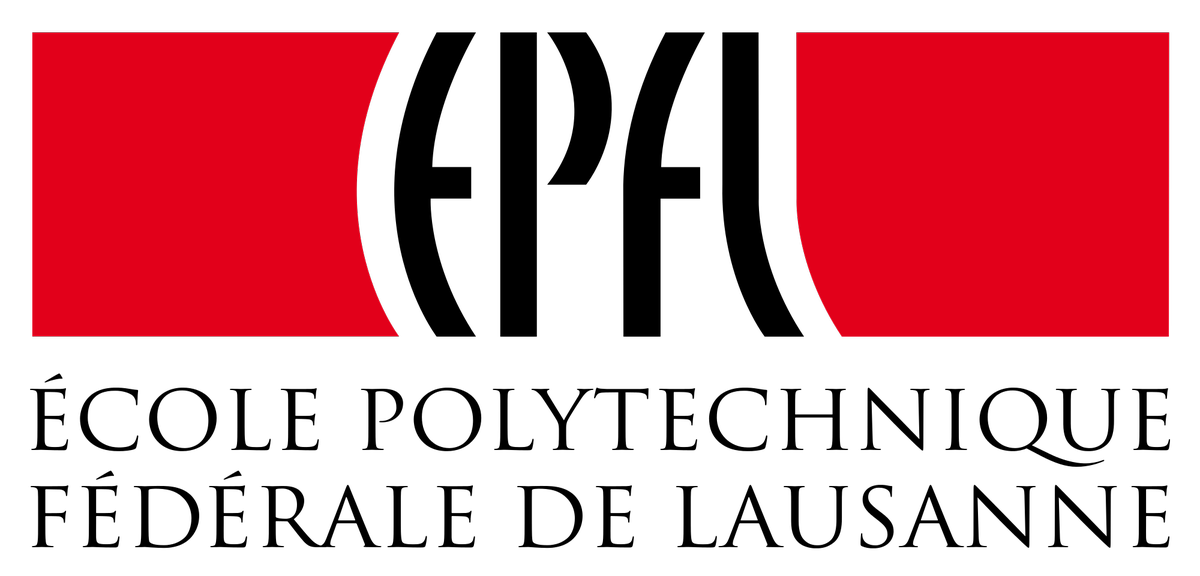
\includegraphics[width=7cm]{epfl-logo}

       \vfill
   \end{center} 
\end{titlepage} 
\setcounter{chapter}{2}
\chapter{Dynamique}
\label{cha:dynamique}

\section{Première loi de Newton}

\begin{highlightBox}
    Un objet a un mouvement rectiligne uniforme (MRU), ainsi $\vec v = \vec{cste}$ et
    $\vec a = \vec 0$  si et seulement si il ne subir aucune action
    extérieure. (force extérieure résultante est nulle)
\end{highlightBox}

\paragraph{Exemple:}

Un pock qui glace à vitesse constante $\vec v = \vec{cste}$ sur la glace d'une
patinoire.

\paragraph{Référentiel d'inertie}

Tout référentiel par rapport auquel le principe d'inertie est vérifié.

\paragraph{Exemple:}

La patinoire est un référentiel d'inertie pour le pock.

\paragraph{Contre-exemple:}

La patinoire qui est en rotation autour d'un axe vectoriel. Le pock bouge par
rapport à la patinoire sans qu'on agisse sur lui.

\section{Deuxième loi de Newton}

\subsection{Force}

\begin{description}
    \item[Force] $(\vec F)$ grandeur physique qui modifie l'état de mouvement
        rectiligne uniforme (MRU) d'un objet.
    \item Grandeur extensive
    \item Grandeur vectorielle
\end{description}

\pagebreak

La force satisfait la règle d'addition vectorielle (règle du parallélogramme)

\begin{center}
    \begin{minipage}{.5\linewidth}
        \resizebox{\textwidth}{!}{
            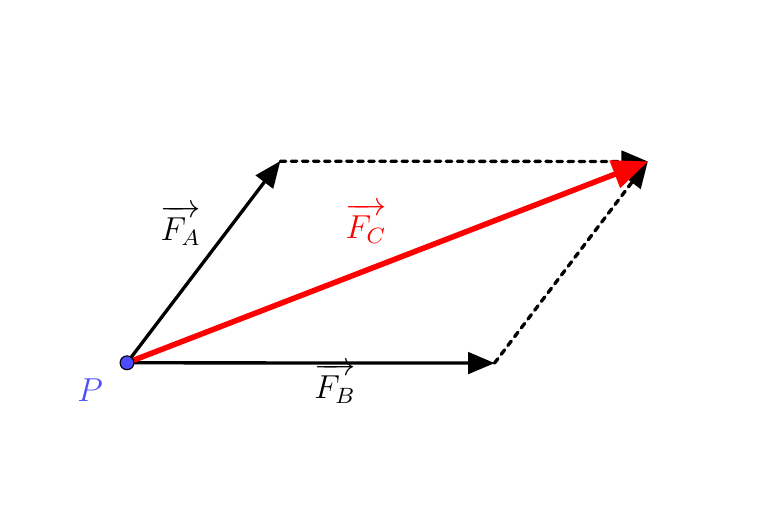
\begin{tikzpicture}[line cap=round,line join=round,>=triangle 45,x=1.0cm,y=1.0cm]
            \clip(-5.,-3.) rectangle (4.,3.);
            \draw [->,line width=1.2pt] (-3.7384198614380675,-1.255971691979606) -- (-1.7924839175732676,1.3044703394214465);
            \draw [->,line width=1.2pt] (-3.7384198614380675,-1.255971691979606) -- (0.9289,-1.26);
            \draw [->,line width=1.2pt,dash pattern=on 2pt off 2pt] (0.9289,-1.26) -- (2.8748359438647997,1.3004420314010525);
            \draw [->,line width=1.2pt,dash pattern=on 2pt off 2pt] (-1.7924839175732676,1.3044703394214463) -- (2.8748359438647997,1.3004420314010523);
            \draw [->,line width=2.pt,color=ffqqqq] (-3.7384198614380675,-1.255971691979606) -- (2.8748359438647992,1.3004420314010525);
            \begin{scriptsize}
            \draw [fill=ududff] (-3.7384198614380675,-1.255971691979606) circle (2.5pt);
            \draw[color=ududff] (-4.206614975751404,-1.5998024790534608) node {$P$};
            \draw[color=black] (-3.058073835951503,0.4851288893731105) node {$\vec{F_A}$};
            \draw[color=black] (-1.0975067947644108,-1.5193314437808565) node {$\vec{F_B}$};
            \draw[color=ffqqqq] (-0.7024671670625339,0.514391084017694) node {$\vec{F_C}$};
            \end{scriptsize}
            \end{tikzpicture}
        }
    \end{minipage}
    \begin{minipage}{.49\linewidth}
        \setlength{\parskip}{.3em}
        $$\vec{F_{A}} + \vec{F_{B}} = \vec{F_{C}}$$
    \end{minipage}
\end{center}


Unité physique (SI): newton $[N] \quad [kg \cdot \frac{m}{s^{2}}]$ 


\subsection{Deuxième loi de Newton}
\label{sub:deuxieme_loi_de_newton}

\begin{highlightBox}
    \begin{center}
        Un objet a un mouvement accéléré ($\vec v = \vec{cste}$ et $ \vec a = \vec 0$)
    \end{center}
\end{highlightBox}

Mathématiquement, on l'écrit:

\begin{equation}
    \label{eq:3.1}
    \cfbox{red}{ $\vec F = m \cdot \vec a$ }
\end{equation}

où ici $\vec F$ est la résultante des forces extérieure qui s'exercent sur
l'objet.

\paragraph{Remarques:}

\begin{itemize}
    \item La force est la cause, l'accélération est l'effet: l'objet de masse
        $m$ subit une force $\vec F$ génère une accélération $\vec a$.
    \item Les vecteurs $\vec{a}$ et $\vec F$ sont parallèles et de même sens (i.e.
        $m > 0$)
    \item Plus la masse $m$ de l'objet est grande, plus il est difficile de
        l'accéléré, c'est à dire de modifier sa vitesse.
\end{itemize}

\paragraph{Remarques générales:}


\begin{enumerate}
    \item Une force qui est opposée à la vitesse (triangle) va provoquer un
        ralentissement l'accélération $\vec a$ est opposé à la vitesse $\vec v$
    \item Une force non-parallèle à la vitesse (force latéral) provoque un
        virage. La force est orientée vers l'intérieur du virage.
    \item Si un objet est au repos, la résultante des forces que cet objet
        subit est nulle:
        \begin{highlightBox}
            $$ \text{ Objet statique } (\vec v = \vec 0) \implies \vec F = \vec 0, \quad \forall t $$
        \end{highlightBox}

        \Warning La réciproque est fausse: si l'objet ne subit aucune force
        résultante, il n'est pas nécessairement au repos (MRU)
\end{enumerate}


\begin{highlightBox}[frametitle={Méthodologie}]
    Pour appliquer la deuxième loi de Newton dans un problème spécifique, il
    est recommandé de procéder de la manière suivante:
    \begin{enumerate}
        \item Faire une dessin
        \item Choisir un référentiel d'inertie
        \item Désigner l'objet considérée
        \item Identifier toutes les forces extérieures exercées sur l'objet
        \item Écrire la deuxième loi de Newton (vectoriellement)
        \item Choisir un repère
        \item Faire des projections
    \end{enumerate}
\end{highlightBox}

\section{Forces particulières}
\label{sec:forces_particulieres}

\subsection{Forces à distances}
\label{sub:forces_a_distances}

Elles sont exercées sans contact avec l'objet considéré.

\begin{enumerate}
    \item \textbf{Force de la gravitation:}  les masses s'attirent 
        \begin{center}
            \begin{minipage}{.5\linewidth}
                \resizebox{\textwidth}{!}{
                    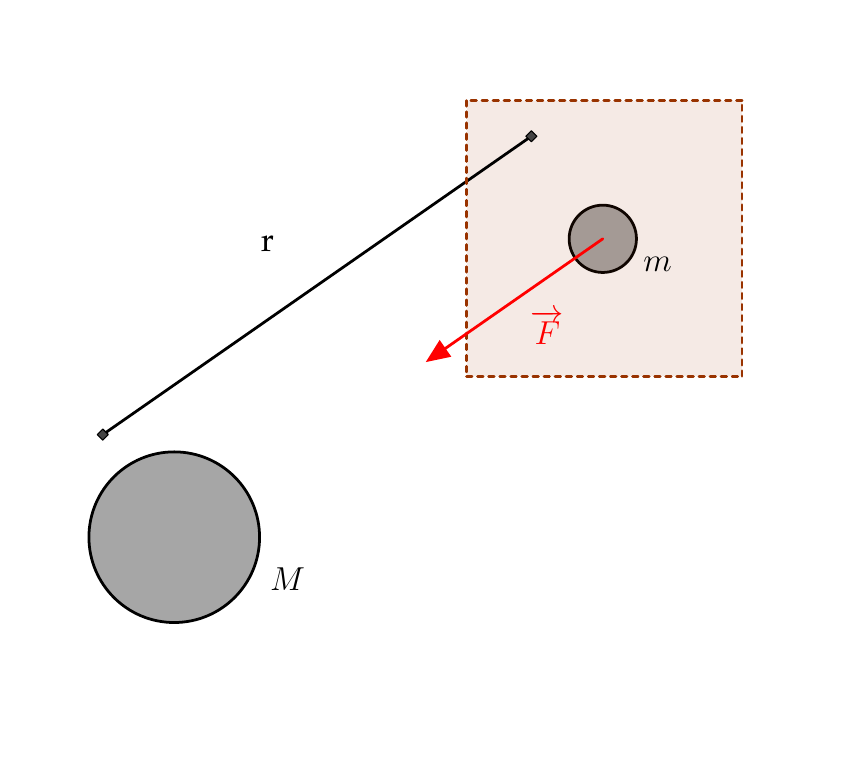
\begin{tikzpicture}[line cap=round,line join=round,>=triangle 45,x=1.0cm,y=1.0cm]
                        \clip(-5.,-2.) rectangle (5.,7.);
                        \draw [line width=1.pt,fill=black,fill opacity=0.3499999940395355] (-3.1385448712241075,0.5290221813399866) circle (1.0835905654656801cm);
                        \draw [line width=1.pt,fill=black,fill opacity=0.3499999940395355] (2.304223332668417,4.318476387813545) circle (0.4273182239886096cm);
                        \fill[line width=1pt,dash pattern=on 2pt off 2pt,color=zzttqq,fill=zzttqq,fill opacity=0.10000000149011612] (0.5731554866114585,6.073155486611459) -- (0.5731554866114585,2.5731554866114594) -- (4.0731554866114585,2.5731554866114594) -- (4.0731554866114585,6.073155486611459) -- cycle;
                        \draw [line width=1.pt] (-4.045688865591133,1.831947146222355)-- (1.3970793383013915,5.621401352695914);
                        \draw [line width=1.pt,dash pattern=on 2pt off 2pt,color=zzttqq] (0.5731554866114585,6.073155486611459)-- (0.5731554866114585,2.5731554866114594);
                        \draw [line width=1.pt,dash pattern=on 2pt off 2pt,color=zzttqq] (0.5731554866114585,2.5731554866114594)-- (4.0731554866114585,2.5731554866114594);
                        \draw [line width=1.pt,dash pattern=on 2pt off 2pt,color=zzttqq] (4.0731554866114585,2.5731554866114594)-- (4.0731554866114585,6.073155486611459);
                        \draw [line width=1.pt,dash pattern=on 2pt off 2pt,color=zzttqq] (4.0731554866114585,6.073155486611459)-- (0.5731554866114585,6.073155486611459);
                        \draw [->,line width=1.pt,color=ffqqqq] (2.304223332668417,4.318476387813545) -- (0.05564471291057593,2.7529337466380586);
                        \begin{scriptsize}
                        \draw [fill=uuuuuu] (-4.045688865591133,1.831947146222355) ++(-2.0pt,0 pt) -- ++(2.0pt,2.0pt)--++(2.0pt,-2.0pt)--++(-2.0pt,-2.0pt)--++(-2.0pt,2.0pt);
                        \draw [fill=uuuuuu] (1.3970793383013915,5.621401352695914) ++(-2.0pt,0 pt) -- ++(2.0pt,2.0pt)--++(2.0pt,-2.0pt)--++(-2.0pt,-2.0pt)--++(-2.0pt,2.0pt);
                        \draw[color=black] (-1.954635169715365,4.260979802881739) node {r};
                        \draw[color=ffqqqq] (1.600721479601531,3.192909698354441) node {$\vec F$};
                        \draw[color=black] (-1.7,0) node {$M$};
                        \draw[color=black] (3,4) node {$m$};
                        \end{scriptsize}
                    \end{tikzpicture}
                }
            \end{minipage}
            \begin{minipage}{.49\linewidth}
                \setlength{\parskip}{.3em}

                \begin{equation}
                    \label{eq:3.2}
                    || \vec F || = G \cdot \frac{M \cdot m}{r^{2}} 
                \end{equation}

                \begin{itemize}
                    \item Force proportionnelle au produit des masses
                    \item Force inversement proportionnelle au carré de la
                        distance qui les séparent.
                \end{itemize}
            \end{minipage}
        \end{center}

        $$G = 6.67 \cdot 10^{-11} \frac{N \cdot m^{2}}{kg^{2}}: \text{
        constante universelle de la gravitation}$$

        \paragraph{Exemples:}

        \begin{itemize}
            \item La terre est attirée par le soleil
            \item La soleil est attirée par le terre 
        \end{itemize}

        Près de la surface de la terre, le champ gravitationnel a une norme $g =
        \frac{G \cdot M}{r^{2}}$  qui est quasiment constant (car $r = cst$). Dans ce
        cas, la force de gravitation est appelé le \textbf{poids}.


        \begin{center}
            \begin{minipage}{.5\linewidth}
                \resizebox{\textwidth}{!}{
                        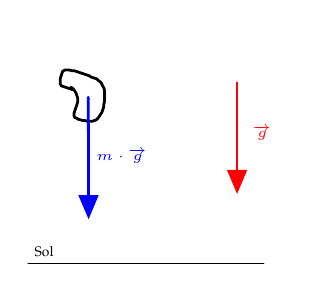
\begin{tikzpicture}[line cap=round,line join=round,>=triangle 45,x=1.0cm,y=1.0cm]
                        \clip(1.,1.) rectangle (4.5,4.);
                        \draw[line width=1pt] (1.5488927444371998,3.245036582569775) -- (1.5809964263788354,3.2209588211135483) -- (1.5970482673496533,3.196881059657321) -- (1.6131001083204712,3.1728032982010945) -- (1.62112602880588,3.148725536744868) -- (1.6291519492912891,3.1246477752886412) -- (1.6371778697766979,3.100570013832414) -- (1.6371778697766979,3.0684663318907788) -- (1.6291519492912891,3.036362649949143) -- (1.62112602880588,3.0122848884929163) -- (1.6131001083204712,2.9882071270366892) -- (1.605074187835062,2.9641293655804626) -- (1.5970482673496533,2.940051604124236) -- (1.5890223468642446,2.9159738426680093) -- (1.5890223468642446,2.8838701607263735) -- (1.5970482673496533,2.859792399270147) -- (1.62112602880588,2.8517664787847377) -- (1.645203790262107,2.83571463781392) -- (1.6773074722037424,2.827688717328511) -- (1.701385233659969,2.8196627968431023) -- (1.733488915601605,2.8196627968431023) -- (1.7575666770578315,2.811636876357693) -- (1.7896703589994674,2.811636876357693) -- (1.8217740409411032,2.811636876357693) -- (1.8458518023973298,2.8196627968431023) -- (1.8699295638535565,2.827688717328511) -- (1.894007325309783,2.8517664787847377) -- (1.910059166280601,2.8758442402409647) -- (1.926111007251419,2.8999220016971914) -- (1.9421628482222368,2.923999763153418) -- (1.9501887687076456,2.9480775246096447) -- (1.9582146891930547,2.9721552860658718) -- (1.9662406096784635,2.9962330475220984) -- (1.9662406096784635,3.0283367294637342) -- (1.9742665301638724,3.052414490919961) -- (1.9742665301638724,3.0845181728615962) -- (1.9742665301638724,3.116621854803232) -- (1.9742665301638724,3.148725536744868) -- (1.9742665301638724,3.1808292186865037) -- (1.9742665301638724,3.212932900628139) -- (1.9662406096784635,3.2370106620843657) -- (1.9501887687076456,3.261088423540593) -- (1.9421628482222368,3.2851661849968194) -- (1.926111007251419,3.309243946453046) -- (1.9020332457951923,3.325295787423864) -- (1.8779554843389656,3.3493735488800906) -- (1.8538777228827386,3.3573994693655) -- (1.829799961426512,3.3654253898509086) -- (1.8057221999702853,3.3734513103363177) -- (1.7816444385140586,3.389503151307135) -- (1.7575666770578315,3.3975290717925444) -- (1.733488915601605,3.405554992277953) -- (1.7094111541453783,3.4135809127633623) -- (1.6853333926891516,3.421606833248771) -- (1.6612556312329245,3.4296327537341798) -- (1.6371778697766979,3.437658674219589) -- (1.6131001083204712,3.4456845947049977) -- (1.5890223468642446,3.453710515190407) -- (1.5569186649226088,3.453710515190407) -- (1.532840903466382,3.4617364356758156) -- (1.5007372215247463,3.4617364356758156) -- (1.4686335395831107,3.4617364356758156) -- (1.4445557781268838,3.4456845947049977) -- (1.436529857641475,3.421606833248771) -- (1.428503937156066,3.3975290717925444) -- (1.4204780166706572,3.3734513103363177) -- (1.4124520961852483,3.3493735488800906) -- (1.4124520961852483,3.3172698669384553) -- (1.4124520961852483,3.2851661849968194) -- (1.428503937156066,3.261088423540593) -- (1.4525816986122928,3.2530625030551836) -- (1.4766594600685194,3.245036582569775) -- (1.5007372215247463,3.2370106620843657) -- (1.524814982980973,3.228984741598957) -- (1.5488927444371998,3.2209588211135483) -- (1.5729705058934267,3.212932900628139);
                        \draw [->,line width=1.pt,color=qqqqff] (1.77,3.11662) -- (1.7736185180286492,1.5676192011193106);
                        \draw [->,line width=1.pt,color=ffqqqq] (3.659709832099745,3.301218025967637) -- (3.659709832099745,1.8886560205356673);
                        \begin{scriptsize}
                        \draw (4, 1) -- (1, 1) node [anchor=south west] {\tiny Sol} ;
                        \draw[color=qqqqff] (2.1932962122013345,2.3655962678878475) node {\tiny$m \cdot \vec g$};
                        \draw[color=ffqqqq] (3.980187281098314,2.656937203034094) node {\tiny$\vec g$};
                        \end{scriptsize}
                        \end{tikzpicture}
                }
            \end{minipage}
            \begin{minipage}{.49\linewidth}
                \setlength{\parskip}{.3em}

                \begin{equation}
                    \vec F = m \cdot \vec g
                \end{equation}
                où $\vec g$ est dirigé vers le centre de la terre et $|| \vec g || = g
                \approx 9.81 \frac{m}{s^{2}}$ 
            \end{minipage}
        \end{center}

        \paragraph{Exemple:}

        Objet en chute libre, la seul force que subit cet objet, c'est son poids.
        Alors $$\vec F = m \cdot \vec a \implies m \cdot \vec g = m \cdot \vec a
        \implies \vec a (t) = \vec g = \vec{cste}, \quad \forall t$$

        \paragraph{Remarques:}

        \begin{itemize}
            \item L'accélération est constant et égale à $\vec g$ (MUA)
            \item L'accélération est indépendante de la masse.
        \end{itemize}

    \item \textbf{Forces électrique}: les charges électrique de signes opposé
        s'attirent et les charges électriques de même signe se repoussent.

    \item \textbf{Force magnétique}: Une charge électrique en mouvement est
        dérivée par un courant électriques.
\end{enumerate}

\subsection{Forces de contact}
\label{sub:forces_de_contact}

Les forces de contact sont exercées par traction (tension dans un fil), par
pression (soutien d'une table) ou par cisaillement (frottement). Elles sont
transmission par contact avec l'objet considéré.

\begin{description}
    \item[Tension:] pendule simple constitué d'une boule suspendue à un fil
        attaché au plafond.

        \begin{center}
            \begin{minipage}{.5\linewidth}
                \resizebox{\textwidth}{!}{
                    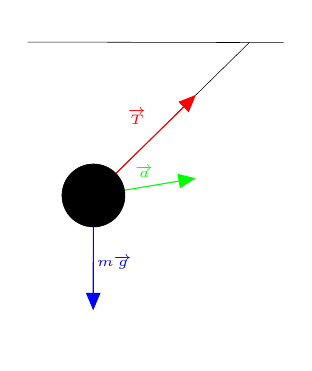
\begin{tikzpicture}[line cap=round,line join=round,>=triangle 45,x=1.0cm,y=1.0cm,
                        scale=.5]
                    \clip(-3.5,-2.) rectangle (3.,6.);
                    \draw [line width=0.2pt,domain=-3.5:3.] plot(\x,{(--32.031402570926375-0.013086077175436195*\x)/5.692443571314553});
                    \draw [line width=0.2pt] (-1.8290956691281008,1.7380232630513102)-- (2.129648603106053,5.622108225406441);
                    \draw [->,line width=0.4pt,color=ffqqqq] (-1.2580511114031636,2.29829829648822) -- (0.7730616344349746,4.291105593562126) node [midway, anchor= south east, font=\tiny]{$\vec T$};
                    \draw [->,line width=0.4pt,color=qqqqff] (-1.8309347447283832,0.9380253769285172) -- (-1.835797047338877,-1.1770762586362402);
                    \draw [->,line width=0.4pt,color=qqffqq] (-1.8290956691281008,1.7380232630513102) -- (0.7681993318244811,2.1760039579973682) node [midway, anchor=south, font=\tiny]{$\vec a$};
                    \draw [line width=0.2pt,fill=black,fill opacity=1.0] (-1.8290956691281008,1.7380232630513102) circle (0.8cm);
                    \begin{scriptsize}
                    \draw[color=black] (-8.211186266638506,5.53224218962704) node {$f$};
                    \draw[color=ffqqqq] (-0.6700744954818247,3.5070091157137835);
                    \draw[color=qqqqff] (-1.295756258154214,0.03282880192762708) node [font=\tiny]{$m \vec g$};
                    \draw[color=qqffqq] (0.10379505308665465,2.222714971280986);
                    \end{scriptsize}
                    \end{tikzpicture}
                }
            \end{minipage}
            \begin{minipage}{.49\linewidth}
                \setlength{\parskip}{.3em}
                \begin{itemize}
                    \item \textbf{Loi du mouvement:} 
                        \begin{equation}
                            m\cdot \vec g + \vec T = m \cdot \vec a
                        \end{equation}
                    \item À chaque instant la somme des forces tend à ramener
                        le pendule à la position verticale. Il s'en suit un
                        mouvement d'oscillation.
                \end{itemize}
            \end{minipage}
        \end{center}

    \item [Soutien:] Une boite qui glisse sur une table est soumise à son poids
        $m\vec g$, à la force de soutien $\vec S$ de la table et à une force
        de frottement $\vec f$ qui s'oppose au mouvement.

        \begin{center}
            \begin{minipage}{.5\linewidth}
                \resizebox{\textwidth}{!}{
                    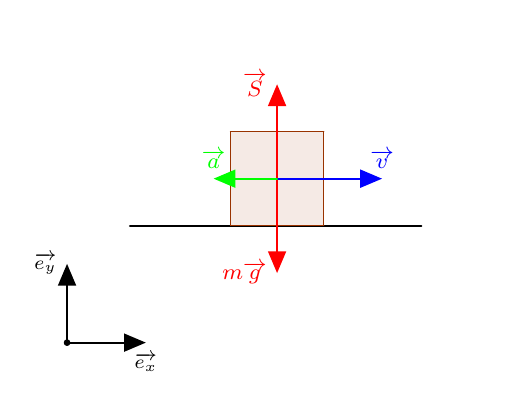
\begin{tikzpicture}[line cap=round,line join=round,>=triangle 45,x=1.0cm,y=1.0cm]
\clip(-0.5,-0.5) rectangle (5.5,4.);
                    \fill[line width=0.4pt,color=zzttqq,fill=zzttqq,fill opacity=0.10000000149011612] (2.0739188156452064,2.675870036301062) -- (3.2610757732995923,2.675870036301062) -- (3.2610757732995923,1.4887130786466765) -- (2.0739188156452064,1.4887130786466765) -- cycle;
                    \draw [->,line width=0.8pt] (0.,0.) -- (0.,1.) node [anchor=east, font=\scriptsize] {$\vec{e_y}$};
                    \draw [->,line width=0.8pt] (0.,0.) -- (1.,0.) node [anchor=north, font=\scriptsize] {$\vec{e_x}$};
                    \draw [line width=0.8pt] (0.8,1.48)-- (4.5,1.48);
                    
                    \draw [line width=0.4pt,color=zzttqq] (2.0739188156452064,2.675870036301062)-- (3.2610757732995923,2.675870036301062);
                    \draw [line width=0.4pt,color=zzttqq] (3.2610757732995923,2.675870036301062)-- (3.2610757732995923,1.4887130786466765);
                    \draw [line width=0.4pt,color=zzttqq] (3.2610757732995923,1.4887130786466765)-- (2.0739188156452064,1.4887130786466765);
                    \draw [line width=0.4pt,color=zzttqq] (2.0739188156452064,1.4887130786466765)-- (2.0739188156452064,2.675870036301062);

                    \draw [->,line width=0.8pt,color=ffqqqq] (2.6674972944723994,2.0822915574738694) -- (2.6674972944723994,3.280766484243587) node [anchor=east, font=\footnotesize] {$\vec S$};
                    \draw [->,line width=0.8pt,color=ffqqqq] (2.6674972944723994,2.0822915574738694) -- (2.6674972944723994,0.8838166307041522) node [anchor=east, font=\footnotesize] {$m \vec g$};
                    \draw [->,line width=0.8pt,color=qqqqff] (2.6674972944723994,2.0822915574738694) -- (4.,2.0822915574738694) node [anchor=south, font=\footnotesize] {$\vec v$};
                    \draw [->,line width=0.8pt,color=qqffqq] (2.6674972944723994,2.0822915574738694) -- (1.8620070751596762,2.0822915574738694) node [anchor=south, font=\footnotesize] {$\vec a$};
                    \begin{scriptsize}
                    \draw [fill=black] (0.,0.) circle (1.0pt);
                    \end{scriptsize}
                    \end{tikzpicture}
                }
            \end{minipage}
            \begin{minipage}{.49\linewidth}
                \setlength{\parskip}{.3em}
                \textbf{Loi de mouvement:} $$m \cdot \vec g + \vec S + \vec f
                = m \cdot \vec a$$
                Projections sur les axes:
                \begin{equation}
                    \begin{split}
                        \text{ selon } \vec{e_{x}}&: -f = m \cdot (-a)\\
                        \text{ selon } \vec{e_{y}}&: -m \cdot g + S = 0
                    \end{split}
                \end{equation}
            \end{minipage}
        \end{center}

        Comme la boite ne quitte pas la table, l'accélération est parallèles à
        la table. Ainsi,
        \begin{equation}
            \left\{
                \begin{array}{l}
                f = m \cdot a\\
                S = m \cdot g
                \end{array}
            \right.
        \end{equation}

    \item[Traction:] Une locomotive pousse un wagon avec une force de traction
        $\vec T$. Le wagon a un masse $m$ et le frottement est négligeable.

        \begin{center}
            \begin{minipage}{.5\linewidth}
                \resizebox{\textwidth}{!}{
                    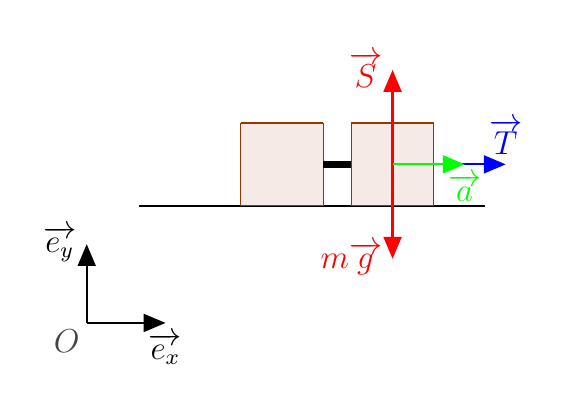
\begin{tikzpicture}[line join=round,>=triangle 45,x=1.0cm,y=1.0cm]
                    \clip(-0.75,-0.75) rectangle (6.,3.75);
                    \fill[line width=0.4pt,color=zzttqq,fill=zzttqq,fill opacity=0.10000000149011612] (3.3588228466203756,2.5390187721884008) -- (4.4091285401621,2.5390187721884003) -- (4.4091285401621,1.4887130786466765) -- (3.3588228466203756,1.4887130786466765) -- cycle;
                    \fill[line width=0.4pt,color=zzttqq,fill=zzttqq,fill opacity=0.10000000149011612] (3.0056227018895303,2.5390187721884008) -- (1.955317008347806,2.5390187721884003) -- (1.955317008347806,1.4887130786466762) -- (3.0056227018895303,1.4887130786466765) -- cycle;
                    \draw [->,line width=0.8pt] (0.,0.) -- (0.,1.) node [anchor = east]{$\vec{e_y}$};
                    \draw [->,line width=0.8pt] (0.,0.) -- (1.,0.) node [anchor = north]{$\vec{e_x}$};
                    \draw [line width=0.8pt] (0.6642059142479815,1.4887130786466765)-- (5.060839052761469,1.4887130786466765);
                    \draw [line width=0.4pt,color=zzttqq] (3.3588228466203756,2.5390187721884008)-- (4.4091285401621,2.5390187721884003);
                    \draw [line width=0.4pt,color=zzttqq] (4.4091285401621,2.5390187721884003)-- (4.4091285401621,1.4887130786466765);
                    \draw [line width=0.4pt,color=zzttqq] (4.4091285401621,1.4887130786466765)-- (3.3588228466203756,1.4887130786466765);
                    \draw [line width=0.4pt,color=zzttqq] (3.3588228466203756,1.4887130786466765)-- (3.3588228466203756,2.5390187721884008);

                    \draw [->,line width=0.8pt,color=ffqqqq] (3.8839756933912377,2.013865925417538) -- (3.8839756933912377,3.2123408521872556) node [anchor= east] {$\vec S$};
                    \draw [->,line width=0.8pt,color=ffqqqq] (3.8839756933912377,2.013865925417538) -- (3.8839756933912377,0.8153909986478212) node [anchor= east] {$m\vec g$};
                    \draw [->,line width=0.8pt,color=qqqqff] (3.8839756933912377,2.013865925417538) -- (5.3200131239416475,2.013865925417538) node [anchor= south] {$\vec T$};
                    \draw [->,line width=0.8pt,color=qqffqq] (3.8839756933912377,2.013865925417538) -- (4.799507647496192,2.013865925417538) node [anchor= north] {$\vec a$};

                    \draw [line width=0.4pt,color=zzttqq] (3.0056227018895303,2.5390187721884008)-- (1.955317008347806,2.5390187721884003);
                    \draw [line width=0.4pt,color=zzttqq] (1.955317008347806,2.5390187721884003)-- (1.955317008347806,1.4887130786466762);
                    \draw [line width=0.4pt,color=zzttqq] (1.955317008347806,1.4887130786466762)-- (3.0056227018895303,1.4887130786466765);
                    \draw [line width=0.4pt,color=zzttqq] (3.0056227018895303,1.4887130786466765)-- (3.0056227018895303,2.5390187721884008);

                    \draw [line width=2.8pt] (3.0056227018895303,2.0138659254175377)-- (3.358822846620375,2.0138659254175377);
                    \begin{scriptsize}
                    \draw[color=uuuuuu] (0,0) node [anchor= north east] {$O$};
                    \end{scriptsize}
                    \end{tikzpicture}
                }
            \end{minipage}
            \begin{minipage}{.49\linewidth}
                \setlength{\parskip}{.3em}
                \textbf{Loi du mouvement:} 
                $$m \cdot \vec g + \vec S + \vec T = m \cdot \vec a$$
                \begin{equation}
                    \begin{split}
                        \text{ selon } \vec{e_{x}}&: T = m \cdot a\\
                        \text{ selon } \vec{e_{x}}&: -m \cdot g + S = 0
                    \end{split}
                \end{equation}
            \end{minipage}
        \end{center}

        Ainsi,

        $$
        \left\{
            \begin{array}{l}
            T = m\cdot a\\
            S = m\cdot g\\
            \end{array}
        \right.
        $$

    \item[Force élastique] Un ressort est formé d'un tige enroulée en spirale.
        Il a une certaine longueur au repos et un rigidité (difficulté à
        déforme). La force exercée par le ressort est proportionelle à son
        allongement $\vec d$ (vecteur déplacement de l'extrémité).


        \begin{center}
            \begin{minipage}{.5\linewidth}
                \resizebox{\textwidth}{!}{
                    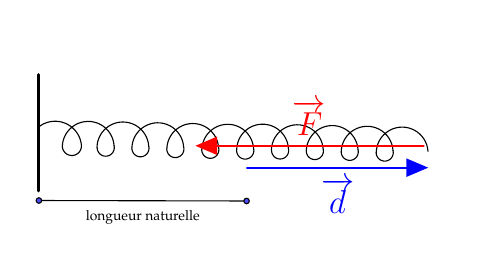
\begin{tikzpicture}[line cap=round,line join=round,>=triangle 45,x=1.0cm,y=1.0cm]
                    \clip(1.,0.25) rectangle (6.5,3.);
                    \draw [line width=1.2pt] (1.14,2.40226)-- (1.14,0.92895);
                    \draw [shift={(1.7684916352518227,1.4806931399102026)},line width=0.4pt]  plot[domain=0.06500979957568542:3.12202957569739,variable=\t]({1.*0.32906412701674337*cos(\t r)+0.*0.32906412701674337*sin(\t r)},{0.*0.32906412701674337*cos(\t r)+1.*0.32906412701674337*sin(\t r)});
                    \draw [shift={(1.9913452664056495,1.4762363178327993)},line width=0.4pt]  plot[domain=-3.150188430415746:0.24011421226757407,variable=\t]({1.*0.10863194455243587*cos(\t r)+0.*0.10863194455243587*sin(\t r)},{0.*0.10863194455243587*cos(\t r)+1.*0.10863194455243587*sin(\t r)});
                    \draw [shift={(2.209228456851315,1.4732230242898718)},line width=0.4pt]  plot[domain=0.06500979957568677:3.122029575697389,variable=\t]({1.*0.32906412701674315*cos(\t r)+0.*0.32906412701674315*sin(\t r)},{0.*0.32906412701674315*cos(\t r)+1.*0.32906412701674315*sin(\t r)});
                    \draw [shift={(2.4320820880051417,1.468766202212469)},line width=0.4pt]  plot[domain=-3.150188430415746:0.24011421226757407,variable=\t]({1.*0.10863194455243587*cos(\t r)+0.*0.10863194455243587*sin(\t r)},{0.*0.10863194455243587*cos(\t r)+1.*0.10863194455243587*sin(\t r)});
                    \draw [shift={(2.652455316990918,1.463262870129432)},line width=0.4pt]  plot[domain=0.06500979957568542:3.12202957569739,variable=\t]({1.*0.32906412701674315*cos(\t r)+0.*0.32906412701674315*sin(\t r)},{0.*0.32906412701674315*cos(\t r)+1.*0.32906412701674315*sin(\t r)});
                    \draw [shift={(2.8753089481447454,1.4588060480520286)},line width=0.4pt]  plot[domain=-3.150188430415746:0.24011421226757504,variable=\t]({1.*0.10863194455243544*cos(\t r)+0.*0.10863194455243544*sin(\t r)},{0.*0.10863194455243544*cos(\t r)+1.*0.10863194455243544*sin(\t r)});
                    \draw [shift={(3.096503405676745,1.4538512299113484)},line width=0.4pt]  plot[domain=0.06500979957568609:3.1220295756973893,variable=\t]({1.*0.32906412701674315*cos(\t r)+0.*0.32906412701674315*sin(\t r)},{0.*0.32906412701674315*cos(\t r)+1.*0.32906412701674315*sin(\t r)});
                    \draw [shift={(3.319357036830571,1.4493944078339451)},line width=0.4pt]  plot[domain=-3.1501884304157484:0.24011421226757507,variable=\t]({1.*0.10863194455243635*cos(\t r)+0.*0.10863194455243635*sin(\t r)},{0.*0.10863194455243635*cos(\t r)+1.*0.10863194455243635*sin(\t r)});
                    \draw [shift={(3.540843765586731,1.4436754964782954)},line width=0.4pt]  plot[domain=0.065009799575686:3.1220295756973893,variable=\t]({1.*0.3290641270167427*cos(\t r)+0.*0.3290641270167427*sin(\t r)},{0.*0.3290641270167427*cos(\t r)+1.*0.3290641270167427*sin(\t r)});
                    \draw [shift={(3.762950830970745,1.439799336666303)},line width=0.4pt]  plot[domain=-3.2509612181311947:0.2333247745745815,variable=\t]({1.*0.10922151995316001*cos(\t r)+0.*0.10922151995316001*sin(\t r)},{0.*0.10922151995316001*cos(\t r)+1.*0.10922151995316001*sin(\t r)});
                    \draw [shift={(1.348413505143625,1.4760782186916994)},line width=0.4pt]  plot[domain=0.09356021159935966:2.23595340403429,variable=\t]({1.*0.33558225220181703*cos(\t r)+0.*0.33558225220181703*sin(\t r)},{0.*0.33558225220181703*cos(\t r)+1.*0.33558225220181703*sin(\t r)});
                    \draw [shift={(1.5612872733958991,1.4982568261660898)},line width=0.4pt]  plot[domain=-3.047015749358122:0.07551345650922035,variable=\t]({1.*0.1215872910210262*cos(\t r)+0.*0.1215872910210262*sin(\t r)},{0.*0.1215872910210262*cos(\t r)+1.*0.1215872910210262*sin(\t r)});
                    \draw [shift={(3.983383046118403,1.4452838411055555)},line width=0.4pt]  plot[domain=0.06500979957568667:3.122029575697389,variable=\t]({1.*0.3290641270167436*cos(\t r)+0.*0.3290641270167436*sin(\t r)},{0.*0.3290641270167436*cos(\t r)+1.*0.3290641270167436*sin(\t r)});
                    \draw [shift={(4.20623667727223,1.440827019028152)},line width=0.4pt]  plot[domain=-3.1501884304157524:0.24011421226757906,variable=\t]({1.*0.10863194455243645*cos(\t r)+0.*0.10863194455243645*sin(\t r)},{0.*0.10863194455243645*cos(\t r)+1.*0.10863194455243645*sin(\t r)});
                    \draw [shift={(4.424119867717896,1.4378137254852255)},line width=0.4pt]  plot[domain=0.06500979957568617:3.1220295756973893,variable=\t]({1.*0.3290641270167436*cos(\t r)+0.*0.3290641270167436*sin(\t r)},{0.*0.3290641270167436*cos(\t r)+1.*0.3290641270167436*sin(\t r)});
                    \draw [shift={(4.646973498871722,1.4333569034078224)},line width=0.4pt]  plot[domain=-3.150188430415746:0.2401142122675731,variable=\t]({1.*0.10863194455243631*cos(\t r)+0.*0.10863194455243631*sin(\t r)},{0.*0.10863194455243631*cos(\t r)+1.*0.10863194455243631*sin(\t r)});
                    \draw [shift={(4.867346727857499,1.4278535713247853)},line width=0.4pt]  plot[domain=0.06500979957568552:3.12202957569739,variable=\t]({1.*0.3290641270167436*cos(\t r)+0.*0.3290641270167436*sin(\t r)},{0.*0.3290641270167436*cos(\t r)+1.*0.3290641270167436*sin(\t r)});
                    \draw [shift={(5.090200359011325,1.423396749247382)},line width=0.4pt]  plot[domain=-3.150188430415746:0.2401142122675731,variable=\t]({1.*0.10863194455243631*cos(\t r)+0.*0.10863194455243631*sin(\t r)},{0.*0.10863194455243631*cos(\t r)+1.*0.10863194455243631*sin(\t r)});
                    \draw [shift={(5.311394816543325,1.4184419311067007)},line width=0.4pt]  plot[domain=0.06500979957568936:3.122029575697386,variable=\t]({1.*0.3290641270167437*cos(\t r)+0.*0.3290641270167437*sin(\t r)},{0.*0.3290641270167437*cos(\t r)+1.*0.3290641270167437*sin(\t r)});
                    \draw [shift={(5.534248447697152,1.4139851090292985)},line width=0.4pt]  plot[domain=-3.1501884304157484:0.24011421226757507,variable=\t]({1.*0.10863194455243635*cos(\t r)+0.*0.10863194455243635*sin(\t r)},{0.*0.10863194455243635*cos(\t r)+1.*0.10863194455243635*sin(\t r)});
                    \draw [shift={(5.755735176453312,1.4082661976736472)},line width=0.4pt]  plot[domain=0.06500979957569072:3.122029575697385,variable=\t]({1.*0.3290641270167437*cos(\t r)+0.*0.3290641270167437*sin(\t r)},{0.*0.3290641270167437*cos(\t r)+1.*0.3290641270167437*sin(\t r)});
                    \draw [line width=0.4pt] (1.1427291806599529,0.804867114289505)-- (3.7799627469869472,0.7989387226784123)
                    node [midway, anchor=north, font=\tiny] {longueur naturelle};
                    \draw [->,line width=0.8pt,color=ffqqqq] (6.02903,1.5) -- (3.13075,1.5) node [anchor =south, midway]{$\vec F$};
                    \draw [->,line width=0.8pt,color=qqqqff] (3.785759299783661,1.2220870768385126) -- (6.086990760079004,1.2220870768385126) node [anchor =north, midway]{$\vec d$};
                    \begin{scriptsize}
                    \draw [fill=ududff] (1.1427291806599529,0.804867114289505) circle (1.0pt);
                    \draw [fill=ududff] (3.7799627469869472,0.7989387226784123) circle (1.0pt);
                    \end{scriptsize}
                    \end{tikzpicture}
                }
            \end{minipage}
            \begin{minipage}{.49\linewidth}
                \setlength{\parskip}{.3em}
                \begin{itemize}
                    \item Force élastique: 
                        \begin{equation}
                            \vec F = - k \cdot \vec d
                        \end{equation}
                    \item La constante de ressort $k$ mesure sa rigidité.
                    \item Unité physique de $k$: $\left[\frac{N}{kg}\right]$
                \end{itemize}
            \end{minipage}
        \end{center}

    \item[Équilibre] Objet immobile suspendu à un ressort

        \begin{center}
            \begin{minipage}{.5\linewidth}
                \resizebox{\textwidth}{!}{
                    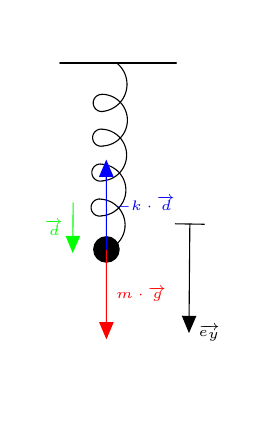
\begin{tikzpicture}[line cap=round,line join=round,>=triangle 45,x=1.0cm,y=1.0cm,rotate=-90, transform shape]
                    \clip(3.25,0.5) rectangle (8.,3.15);
                    \draw [line width=0.4pt,fill=black,fill opacity=1.0] (6.066407810594232,1.5000613949183315) circle (0.1620403061236559cm);
                    \draw [line width=0.8pt] (3.6979177052261782,2.3852072152984922)-- (3.6979177052261782,0.9118972152984922);
                    \draw [shift={(3.969435527566434,1.4153963013513353)},line width=0.4pt]  plot[domain=0.14865391642037343:2.4727127913295393,variable=\t]({1.*0.34613392682680344*cos(\t r)+0.*0.34613392682680344*sin(\t r)},{0.*0.34613392682680344*cos(\t r)+1.*0.34613392682680344*sin(\t r)});
                    \draw [shift={(4.20623667727223,1.440827019028152)},line width=0.4pt]  plot[domain=-3.1501884304157524:0.24011421226757906,variable=\t]({1.*0.10863194455243645*cos(\t r)+0.*0.10863194455243645*sin(\t r)},{0.*0.10863194455243645*cos(\t r)+1.*0.10863194455243645*sin(\t r)});
                    \draw [shift={(4.424119867717896,1.4378137254852255)},line width=0.4pt]  plot[domain=0.06500979957568617:3.1220295756973893,variable=\t]({1.*0.3290641270167436*cos(\t r)+0.*0.3290641270167436*sin(\t r)},{0.*0.3290641270167436*cos(\t r)+1.*0.3290641270167436*sin(\t r)});
                    \draw [shift={(4.646973498871722,1.4333569034078224)},line width=0.4pt]  plot[domain=-3.150188430415746:0.2401142122675731,variable=\t]({1.*0.10863194455243631*cos(\t r)+0.*0.10863194455243631*sin(\t r)},{0.*0.10863194455243631*cos(\t r)+1.*0.10863194455243631*sin(\t r)});
                    \draw [shift={(4.867346727857499,1.4278535713247853)},line width=0.4pt]  plot[domain=0.06500979957568552:3.12202957569739,variable=\t]({1.*0.3290641270167436*cos(\t r)+0.*0.3290641270167436*sin(\t r)},{0.*0.3290641270167436*cos(\t r)+1.*0.3290641270167436*sin(\t r)});
                    \draw [shift={(5.090200359011325,1.423396749247382)},line width=0.4pt]  plot[domain=-3.150188430415746:0.2401142122675731,variable=\t]({1.*0.10863194455243631*cos(\t r)+0.*0.10863194455243631*sin(\t r)},{0.*0.10863194455243631*cos(\t r)+1.*0.10863194455243631*sin(\t r)});
                    \draw [shift={(5.311394816543325,1.4184419311067007)},line width=0.4pt]  plot[domain=0.06500979957568936:3.122029575697386,variable=\t]({1.*0.3290641270167437*cos(\t r)+0.*0.3290641270167437*sin(\t r)},{0.*0.3290641270167437*cos(\t r)+1.*0.3290641270167437*sin(\t r)});
                    \draw [shift={(5.534248447697152,1.4139851090292985)},line width=0.4pt]  plot[domain=-3.1501884304157484:0.24011421226757507,variable=\t]({1.*0.10863194455243635*cos(\t r)+0.*0.10863194455243635*sin(\t r)},{0.*0.10863194455243635*cos(\t r)+1.*0.10863194455243635*sin(\t r)});
                    \draw [shift={(5.755735176453312,1.4082661976736472)},line width=0.4pt]  plot[domain=0.06500979957569072:3.122029575697385,variable=\t]({1.*0.3290641270167437*cos(\t r)+0.*0.3290641270167437*sin(\t r)},{0.*0.3290641270167437*cos(\t r)+1.*0.3290641270167437*sin(\t r)});
                    \draw [->,line width=0.4pt,color=ffqqqq] (6.067108046292919,1.5) -- (7.208749199381812,1.5000613949183312) node [anchor=west, rotate=90, midway, font=\tiny] {$m \cdot \vec g$};
                    \draw [->,line width=0.4pt,color=qqqqff] (6.066407810594232,1.5000613949183315) -- (4.925610348144964,1.4981529124621782)node [anchor = west, rotate=90, midway, font=\tiny] {$-k \cdot \vec{d}$};
                    \draw [line width=0.4pt] (5.746292956158723,2.7425960935623146)-- (5.7407431784626395,2.3763107656207847);
                    \draw [->,line width=0.4pt] (5.743518067310681,2.5594534295915494) -- (7.128187602483585,2.5483538741993823) node [anchor = west, rotate=90, font=\tiny] {$\vec{e_y}$};
                    \draw [->,line width=0.4pt,color=qqffqq] (5.474353849050619,1.0776627847371796) -- (6.112578284100253,1.0721130070410958) node [anchor = east, rotate=90, midway, font=\tiny] {$\vec{d}$};
                    \end{tikzpicture}
                }
            \end{minipage}
            \begin{minipage}{.49\linewidth}
                \setlength{\parskip}{.3em}

                \textbf{Loi du mouvement:} 
                \begin{equation}
                    m \cdot \vec g - k \cdot \vec d = \vec 0
                \end{equation}

                $$\text{ selon } \vec{e_{y}}: m \cdot g - k \cdot d = 0
                \implies d = \frac{m \cdot g}{k}$$
                
                Si la période est faible, alors l'allongement sera faible
                également. Si la constante élastique est grande, alors
                l'allongement sera petit.
            \end{minipage}
        \end{center}
\end{description}



\section{Quantité de mouvement}
\label{sec:quantite_de_mouvement}

\begin{itemize}
    \item On considère un objet de masse $m$ et de vitesse $\vec v$. La
        quantité de mouvement $\vec P$ va s'exprimer comme, 
        \begin{equation}
            \vec P = m \cdot \vec v 
        \end{equation}
    \item C'est une grandeur extensive et vectorielle
    \item Unité physique (SI): $[\frac{kg \cdot m}{s}]$
    \item Pour un objet de masse $m$ constante, la $2^{\text{ème}}$ de Newton
        s'écrit alors:
        \begin{equation}
            \vec F = m \cdot \vec a = m \cdot \dot{\vec v} = \frac{d}{dt} (m
            \cdot \vec v) = \dot{\vec P} \implies \vec F = \dot{\vec P}
        \end{equation}
\end{itemize}


\subsection{Quantité de mouvement}

\begin{itemize}
    \item Come la quantité de mouvement est une grandeur extensive. La
        quantité de mouvement totale $\vec P$ d'un objet formé de $n$ parties
        est la somme des quantité de mouvement de chaque parties.
        \begin{equation}
            \vec P = \vec{P_{1}} +\vec{P_{2}} + ... +\vec{P_{n}}= m_1
            \vec{v_{1}} + m_2 \vec{v_{2}} + ... + m_n \vec{v_{n}} 
        \end{equation}

    \item Comme la force est une grandeur extensive, la force résultante
        totale $\vec F$ exercée sur un objet $N$ parties est la somme des
        forces exercées sur chaque parties.

        \begin{center}
            \begin{minipage}{.4\linewidth}
                \resizebox{\textwidth}{!}{
                    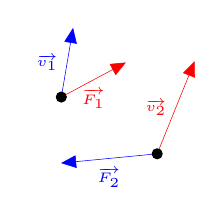
\begin{tikzpicture}[line cap=round,line join=round,>=triangle 45,x=1.0cm,y=1.0cm,scale=0.9]
                    \draw [->,line width=0.2pt,color=qqqqff] (2.8119546964712767,1.3429964890087431) -- (2.977572707641808,2.318302554790762) node[midway, anchor=east, font=\tiny] {$\vec{v_{1}}$};
                    \draw [->,line width=0.2pt,color=ffqqqq] (2.8119546964712767,1.3429964890087431) -- (3.7228537579091996,1.8306495218997525) node[midway, anchor=north, font=\tiny] {$\vec{F_{1}}$};
                    \draw [->,line width=0.2pt,color=ffqqqq] (4.164501787697284,0.542509435017841) -- (4.6914808083375705,1.8456957862216403) node[midway, anchor=east, font=\tiny] {$\vec{v_{2}}$};
                    \draw [->,line width=0.2pt,color=qqqqff] (4.164501787697284,0.542509435017841) -- (2.809011672014314,0.4114335871182065) node[midway, anchor=north, font=\tiny] {$\vec{F_{2}}$};
                    \begin{scriptsize}
                    \draw [fill=black] (2.8119546964712767,1.3429964890087431) circle (2.0pt);
                    \draw [fill=black] (4.164501787697284,0.542509435017841) circle (2.0pt);
                    \end{scriptsize}
                    \end{tikzpicture}
                }
            \end{minipage}
            \begin{minipage}{.59\linewidth}
                \setlength{\parskip}{.3em}
                \begin{equation}
                    \vec F = \vec{F_{1}} + \vec{F_{2}} + ... + \vec{F_{n}}
                \end{equation}

                Objet formé de deux parties:
                \[
                    \begin{split}
                        \text{ partie } 1&: \vec{F_{1}} = m_{1} \cdot \vec{a_{1}}\\
                        \text{ partie } 2&: \vec{F_{2}} = m_{2} \cdot \vec{a_{2}}
                    \end{split}
                \]

                \begin{equation}
                    \vec F = \vec{F_{1}} + \vec{F_{2}} = \frac{d}{dt} (\vec{P_{1}}
                    + \vec{P_{2}}) = \frac{d}{dt} \vec P = \dot{\vec P}
                \end{equation}
            \end{minipage}
        \end{center}
\end{itemize}

\section{Centre de masse}
\label{sec:centre_de_masse}

Dans la $2^e$ loi de Newton: $\vec F = m \cdot \vec a$, l'accélération $\vec a$
est celle de l'objet.  On considère un objet qui est formé de $n$ parties dont
les vecteurs position sont $\vec{r_{i}}$ où $i = 1, 2, ..., n$

\paragraph{Remarque:}

La quantité de mouvement totale s'écrit,

\begin{equation}
    \vec P = m_{1} \cdot \vec{v_{1}} + m_{2} \cdot \vec{v_{2}} + ... + m_{n} \cdot \vec{v_{n}}
    = \frac{d}{dt} (m_{1} \cdot \vec{v_{1}} + m_{2} \cdot \vec{v_{2}} + ... + m_{n} \cdot \vec{v_{n}})
    = \frac{d}{dt} (m \cdot \vec{r_{\text{CM}}}) 
\end{equation}

\paragraph{Centre de masse}
\label{par:centre_de_masse}

\begin{equation}
    \vec{r_{\text{cm}}} = \frac{\vec{r_{1}} + m_{2} \cdot \vec{r_{2}} + ... + m_{n} \cdot \vec{r_{n}}}{m}
\end{equation}
où $m = m_{1} + m_{2} + ... + m_{n} = \text{cste}$ est la masse de l'objet.

Le centre de masse est aussi appelé le centre de gravité. Il coïncide avec le
barycentre (géométrique) si toutes les parties ont une masse identique.

\subsection{Haltère symétrique}
\label{sub:haltere_symetrique}

Le centre de masse (CM) d'une haltère symétrique est à équidistance (milieu)
des 2 masses.

\begin{center}
    \begin{minipage}{.5\linewidth}
        \resizebox{\textwidth}{!}{
            \begin{tikzpicture}[line cap=round,line join=round,>=triangle 45,x=1.0cm,y=1.0cm]
            \clip(-0.5,-0.5) rectangle (13.5,11.5);
            \draw [->,line width=0.8pt] (0.,0.) -- (0.,1.);
            \draw [->,line width=0.8pt] (0.,0.) -- (1.,0.);
            \draw [line width=0.4pt,dash pattern=on 3pt off 3pt] (4.8419352788696,9.899152859754045)-- (11.977766718633058,5.710730058153754);
            \draw [->,line width=0.8pt,color=ffqqqq] (0.009453671837446989,0.) -- (4.8419352788696,9.899152859754045) node [anchor = south east, midway] {$\vec{r_{1}}$};
            \draw [->,line width=0.8pt,color=ffqqqq] (0.009453671837446989,0.) -- (11.977766718633058,5.710730058153754) node [anchor = south east, midway] {$\vec{r_{2}}$};
            \draw [->,line width=0.8pt,color=qqqqff] (0.009453671837446989,0.) -- (8.40985099875133,7.804941458953899) node [anchor = south east, midway] {$\vec{r_{\textsc{cm}}}$};
            \draw [line width=0.4pt] (8.49328035175171,8.045855433347029)-- (4.968485421060643,10.114756805709154) node [midway, anchor=south west] {$\frac{1}{2}$};
            \draw [line width=0.4pt] (8.579521930133051,7.995235376471026)-- (12.104316860824122,5.926334004108897) node [midway, anchor=south west] {$\frac{1}{2}$};
            \begin{scriptsize}
            \draw [fill=black] (4.8419352788696,9.899152859754045) circle (1.0pt) node [anchor= south east] {$m$};
            \draw [fill=black] (11.977766718633058,5.710730058153754) circle (1.0pt) node [anchor= north west] {$m$};
            \end{scriptsize}
            \end{tikzpicture}
        }
    \end{minipage}
    \begin{minipage}{.49\linewidth}
        \setlength{\parskip}{.3em}
        \textbf{Centre de masse} \begin{equation}
            \vec{r_{\textsc{cm}}} = \frac{m \cdot \vec{r_{1}} + m \cdot \vec{r_{2}}}{2m}
            = \frac{1}{2} \cdot (\vec{r_{1}} + \vec{r_{2}})
        \end{equation}
    \end{minipage}
\end{center}

\subsection{Haltère asymétrique}
\label{sub:haltere_asymetrique}

\begin{center}
    \begin{minipage}{.4\linewidth}
        \resizebox{\textwidth}{!}{
            \begin{tikzpicture}[line cap=round,line join=round,>=triangle 45,x=1.0cm,y=1.0cm]
            \clip(-0.5,-0.5) rectangle (14.,12.);
            \draw [->,line width=0.8pt] (0.,0.) -- (0.,1.);
            \draw [->,line width=0.8pt] (0.,0.) -- (1.,0.);
            \draw [->,line width=0.8pt,color=ffqqqq] (0.009453671837446989,0.) -- (11.977766718633058,5.710730058153754) node [anchor = south east, midway] {$\vec{r_{2}}$};
            \draw [->,line width=0.8pt,color=ffqqqq] (0.009453671837446989,0.) -- (4.8419352788696,9.899152859754045) node [anchor = south east, midway] {$\vec{r_{1}}$};
            \draw [line width=0.4pt,dash pattern=on 3pt off 3pt] (4.8419352788696,9.899152859754045)-- (11.977766718633058,5.710730058153754) ;
            \draw [->,line width=0.8pt,color=qqqqff] (0.009453671837446989,0.) -- (9.58970256687446,7.106870992020518) node [anchor = south east, midway] {$\vec{r_{\textsc{cm}}}$};
            \draw [line width=0.4pt] (9.675752271942597,7.351795828017603)-- (4.968485421060643,10.114756805709154) node [midway, anchor=south west] {$\frac{2}{3}$};
            \draw [line width=0.4pt] (9.761597945323404,7.3014081501636525)-- (12.104316860824122,5.926334004108897) node [midway, anchor=south west] {$\frac{1}{3}$};
            \begin{scriptsize}
            \draw [fill=black] (11.977766718633058,5.710730058153754) circle (1.0pt) node [anchor=north west]{$m$};
            \draw[color=black] (12.510835774690445,5.701182054903356);
            \draw [fill=black] (4.8419352788696,9.899152859754045) circle (1.0pt) node [anchor=south east]{$m$};
            \end{scriptsize}
            \end{tikzpicture}
        }
    \end{minipage}
    \begin{minipage}{.59\linewidth}
        \setlength{\parskip}{.3em}
        Le centre de masse (CM) d'une haltère asymétrique n'est pas au milieu
        des masses.

        \begin{equation}
            \vec{r_{\textsc{cm}}} = \frac{m \cdot \vec{r_{1}} + 2 \cdot m \cdot
        \vec{r_{2}}}{3m} = \frac{1}{3} (\vec{r_{1}} + 2 \vec{r_{2}})
        \end{equation}
    \end{minipage}
\end{center}

\begin{itemize}
    \item La quantité de mouvement $\vec P$ d'un objet c'est aussi celle d'une
        masse égale à la masse totale de l'objet située au centre de masse.

        \begin{equation}
            \vec P = \frac{d}{dt} (m \cdot \vec{r_{\textsc{cm}}}) = m \cdot
            \dot{\vec{r_{\textsc{cm}}}} = m \cdot \dot{\vec{v_{\textsc{cm}}}},
            \quad \text{ où } m = \text{ cste } 
        \end{equation}
\end{itemize}

\subsection{Haltère lancée}
\label{sub:haltere_lancee}

Lorsqu'on lance une haltère symétrique, les 2 masses peuvent avoir un
mouvement de rotation propre autour du centre, mais le centre de masse a une
trajectoire balistique.

\begin{center}
    \begin{minipage}{.4\linewidth}
        \resizebox{\textwidth}{!}{
            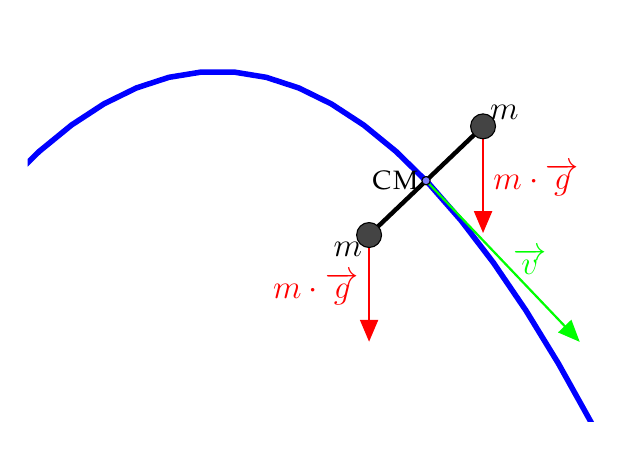
\begin{tikzpicture}[line cap=round,line join=round,>=triangle 45,x=1.0cm,y=1.0cm]
            \clip(4.,3.) rectangle (11.25,8.);
            \draw [samples=50,rotate around={-180.:(6.412013457916292,7.445030598759769)},xshift=6.412013457916292cm,yshift=7.445030598759769cm,line width=2.pt,color=qqqqff,domain=-10.097992667031122:10.097992667031122)] plot (\x,{(\x)^2/2/2.5244981667577804});
            \draw [line width=1.6pt] (8.335809937241638,5.366672139473739)-- (9.783251984374319,6.7468574604332865);
            \draw [->,line width=0.8pt,color=qqffqq] (9.05953096080798,6.0567647999535135) -- (11.010855854100237,4.010351426853534) node [midway, anchor = west]{$\vec v$};
            \draw [->,line width=0.8pt,color=ffqqqq] (8.335809937241638,5.366672139473739) -- (8.335809937241638,4.012228332364821) node [midway, anchor = east]{$m \cdot \vec g$};
            \draw [->,line width=0.8pt,color=ffqqqq] (9.783251984374319,6.7468574604332865) -- (9.783251984374319,5.392413653324369) node [midway, anchor = west]{$m \cdot \vec g$};
            \begin{scriptsize}
            \draw [fill=xdxdff] (9.05953096080798,6.0567647999535135) circle (1.5pt)node
            [anchor = east] {\textsc{cm}};
            \draw [fill=uuuuuu] (8.335809937241638,5.366672139473739) circle (4.5pt) node [anchor= north east] {$m$};
            \draw [fill=uuuuuu] (9.783251984374319,6.7468574604332865) circle (4.5pt) node [anchor= south west] {$m$};
            \end{scriptsize}
            \end{tikzpicture}
        }
    \end{minipage}
    \begin{minipage}{.59\linewidth}
        \setlength{\parskip}{.3em}
        \begin{description}
            \item[Objet:] haltère (masse $2m$)
            \item[Force:] poids: $2 m \cdot \vec g$
            \item[Loi du mouvement:] 
                \begin{equation}
                    2 \cdot m \cdot \vec g = 2 \cdot m \cdot \vec{a_{\textsc{cm}}}
                    \implies \vec{a_{\textsc{cm}}}(t) = \vec g, \quad \forall
                    t 
                \end{equation}
        \end{description}
    \end{minipage}
\end{center}

\paragraph{Remarque:}

\begin{itemize}
    \item Le mouvement du centre de masse est le mouvement global de l'objet (comme
        $m$ de loin)
    \item La $2^e$ loi de Newton ne dit rien sur les mouvements internes à
        l'objet (rotations, vibrations, déformations, ...)
\end{itemize}

\section{Troisième loi de Newton}

\begin{highlightBox}[frametitle={Loi d'action-réaction}]
    La force $\vec{F}_{1\to2}$ exercée par la partie 1 sur la partie 2 d'un
    objet est de même norme, du même support et opposée à la force $\vec{F}_{2\to1}$
    exercée sur la partie 2 sur la partie 1
\end{highlightBox}

\begin{center}
    \begin{minipage}{.5\linewidth}
        \resizebox{\textwidth}{!}{
            \begin{tikzpicture}[line cap=round,line join=round,>=triangle 45,x=1.0cm,y=1.0cm]
            \clip(7.,3.) rectangle (17.,7.);
            \draw [line width=0.2pt,dash pattern=on 3pt off 3pt,domain=7.:17.] plot(\x,{(--66.05802769251785-2.298524917518949*\x)/7.60360305098936});
            \draw [->,line width=0.8pt,color=ffqqqq] (8.47570053419787,6.12557211481141) -- (10.52702173714528,5.505469662435749) node [midway, anchor = south] {$\vec{F}_{1\to2}$};
            \draw [->,line width=0.8pt,color=ffqqqq] (16.07930358518723,3.8270471972924613) -- (14.031470297336853,4.446095273248555) node [midway, anchor = south] {$\vec{F}_{2\to1}$};

            \begin{scriptsize}
            \draw [fill=black] (8.47570053419787,6.12557211481141) circle (3.0pt) node [anchor=north east] {1};
            \draw [fill=black] (16.07930358518723,3.8270471972924613) circle (3.0pt) node [anchor=north west] {2};

            \end{scriptsize}
            \end{tikzpicture}
        }
    \end{minipage}
    \begin{minipage}{.49\linewidth}
        \setlength{\parskip}{.3em}
        
        Mathématiquement, la troisième loi de Newton s'écrit, \begin{equation}
            \vec F_{1\to2} = - \vec F_{2\to1} \implies \vec F_{1\to2} + \vec F_{2\to1}
            = \vec 0
        \end{equation}
    \end{minipage}
\end{center}

\subsection{Deuxième loi de Newton}
\label{sub:deuxieme_loi_de_newton}

\begin{itemize}
    \item On considère un objet constitué de différentes parties qui sont
        soit en contact, soit disjointes.

    \item Compte tenu de la $3^e$ loi de Newton, les forces internes à l'objet
        qui s'exercent entre les parties d'un objets s'annulent deux à deux
        lorsqu'on somme toutes les forces.

    \item Ainsi, seules les forces extérieurs, dont la résultante est notée $\vec F^{\text{est}}$,
        contribuer à modifier la quantité de mouvement totale $\vec P$ de
        l'objet (ou le mouvement du centre de masse).
    \item La $2^e$ loi de Newton s'écrit finalement,
        \begin{equation}
            \vec F^{\text{est}} = \dot{\vec P} = m \cdot \vec{a_{\textsc{cm}}},
            \text{ ou si } m = \text{ cste } 
        \end{equation}

        \paragraph{Remarque:}
        
        En absence de force extérieure résultante, la quantité de mouvement
        totale est constante.
\end{itemize}


\subsection{Choc de 2 chariots sur un rail horizontal}
\label{sub:choc_de_2_chariots_sur_un_rail_horizontal}

\begin{center}
    \begin{minipage}{.5\linewidth}
        \resizebox{\textwidth}{!}{
            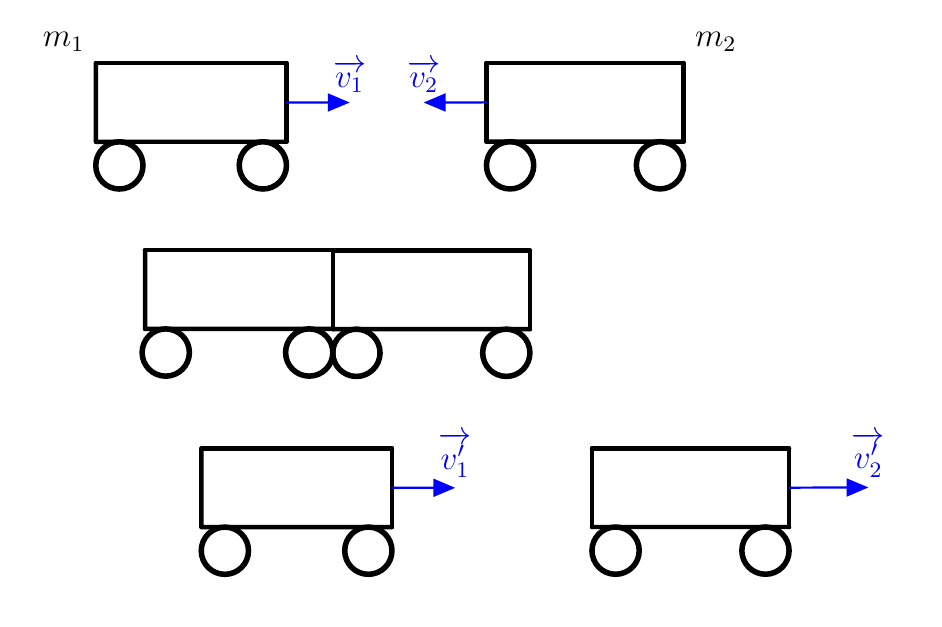
\begin{tikzpicture}[line cap=round,line join=round,>=triangle 45,x=1.0cm,y=1.0cm]
            \clip(10.75,0.) rectangle (22.,7.25);
            \draw [line width=2.pt] (11.914460420800564,5.500686650267401) circle (0.3cm);
            \draw [line width=2.pt] (13.736583021541843,5.501046020207086) circle (0.3cm);
            \draw [line width=2.pt] (16.876479659082925,5.50166528944001) circle (0.3cm);
            \draw [line width=2.pt] (18.77993389770386,5.502040700092755) circle (0.3cm);
            \draw [line width=1.6pt] (11.616863674601857,5.80062796228828)-- (14.036523847910388,5.801105182169186);
            \draw [line width=1.6pt] (16.576420497120758,5.8016061158084735)-- (19.0798747240724,5.802099862054835);
            \draw [line width=1.6pt] (11.616666448612486,6.800627942839233)-- (14.036523847910388,6.800627942839233);
            \draw [line width=1.6pt] (14.036523847910388,6.800627942839233)-- (14.036523847910388,5.801105182169186);
            \draw [line width=1.6pt] (11.616666448612486,6.800627942839233) node [anchor=south east] {$m_{1}$}-- (11.616863674601857,5.80062796228828);

            \draw [line width=1.6pt] (16.576420497120758,6.800627942839233)-- (19.0798747240724,6.800627942839233) node [anchor=south west] {$m_{2}$};
            \draw [line width=1.6pt] (19.0798747240724,6.800627942839233)-- (19.0798747240724,5.802099862054835);
            \draw [line width=1.6pt] (16.576420497120758,6.800627942839233)-- (16.576420497120758,5.8016061158084735);
            \draw [->,line width=0.8pt,color=qqqqff] (14.036523847910388,6.3008665625042095) -- (14.838631733044567,6.299292323898846) node [anchor=south] {$\vec{v_{1}}$};
            \draw [->,line width=0.8pt,color=qqqqff] (16.576420497120758,6.301117029323853) -- (15.78,6.29929) node [anchor=south] {$\vec{v_{2}}$};

            \draw [line width=2.pt] (13.25429912891791,0.6072699976199727) circle (0.3cm);
            \draw [line width=2.pt] (15.076421729659174,0.6076293675596585) circle (0.3cm);
            \draw [line width=2.pt] (18.21631836720026,0.6082486367925813) circle (0.3cm);
            \draw [line width=2.pt] (20.11977260582119,0.6086240474453274) circle (0.3cm);
            \draw [line width=1.6pt] (12.956702382719204,0.9072113096408255)-- (15.37636255602772,0.9076885295218073);
            \draw [line width=1.6pt] (17.91625920523822,0.9081894631611725)-- (20.419713432189486,0.9086832094076118);
            \draw [line width=1.6pt] (12.956505156729802,1.907211290191779)-- (15.37636255602772,1.907211290191779);
            \draw [line width=1.6pt] (15.37636255602772,1.907211290191779)-- (15.37636255602772,0.9076885295218073);
            \draw [line width=1.6pt] (12.956505156729802,1.907211290191779)-- (12.956702382719204,0.9072113096408255);
            \draw [line width=1.6pt] (17.91625920523822,1.907211290191779)-- (20.419713432189486,1.907211290191779);
            \draw [line width=1.6pt] (20.419713432189486,1.907211290191779)-- (20.419713432189486,0.9086832094076118);
            \draw [line width=1.6pt] (17.91625920523822,1.907211290191779)-- (17.91625920523822,0.9081894631611725);
            \draw [->,line width=0.8pt,color=qqqqff] (15.37636255602772,1.4074499098567932) -- (16.178470441161906,1.4058756712514175)node [anchor=south] {$\vec{v'_{1}}$};
            \draw [->,line width=0.8pt,color=qqqqff] (20.419713432189486,1.4079472497996954) -- (21.426342779693748,1.4108900577633405)node [anchor=south] {$\vec{v'_{2}}$};
            \draw [line width=2.pt] (12.503377114284843,3.124240111533519) circle (0.3cm);
            \draw [line width=2.pt] (14.325499715026117,3.1245994814732048) circle (0.3cm);
            \draw [line width=1.6pt] (12.240672006537267,3.4241883050924566)-- (14.625440541394532,3.424658643435275);
            \draw [line width=1.6pt] (12.240474780547911,4.424188285643413)-- (14.625440541394532,4.424188285643413);
            \draw [line width=1.6pt] (14.625440541394532,4.424188285643413)-- (14.625440541394532,3.424658643435275);
            \draw [line width=1.6pt] (12.240474780547911,4.424188285643413)-- (12.240672006537267,3.4241883050924566);
            \draw [line width=2.pt] (14.92486918179424,3.120696242293776) circle (0.3cm);
            \draw [line width=2.pt] (16.828323420415174,3.121071652946522) circle (0.3cm);
            \draw [line width=1.6pt] (14.624810019832069,3.420637068662295)-- (17.12826424678359,3.4211308149086728);
            \draw [line width=1.6pt] (14.624810019832069,4.419665777231079)-- (17.12826424678359,4.419665777231079);
            \draw [line width=1.6pt] (17.12826424678359,4.419665777231079)-- (17.12826424678359,3.4211308149086728);
            \draw [line width=1.6pt] (14.624810019832069,4.419665777231079)-- (14.624810019832069,3.420637068662295);
            \end{tikzpicture}
        }
    \end{minipage}
    \begin{minipage}{.49\linewidth}
        \setlength{\parskip}{.3em}

        \begin{description}
            \item[Objet:] deux chariots de masse $m_{1}$ et $m_{2}$
            \item[Forces extérieures:] poids $m_{1} \cdot \vec g$ et $m_{2} \cdot \vec g$,
                forces de soutiens $\vec{S_{1}}$ et $\vec{S_{2}}$ qui se
                comprennent: $$m_{1} \cdot \vec g + \vec{S_{1}} + m_{2} \cdot
                \vec{S_{2}} = \vec 0$$
            \item[Remarque] le mécanisme compliqué du chox ne joue aucun rôle
                (forces internes)
        \end{description}
    \end{minipage}
\end{center}

Comme la force externe résultante est nulle, $\vec{F^{\text{ext}}} = \vec 0$,
la quantité de mouvement totale est constante: $$\vec P = \vec{\text{cste}}$$

\begin{equation}
    \underbrace{m_{1} \cdot \vec{v_{1}} + m_{2} \cdot \vec{v_{2}}}_{\text{avant
    le choc}} = \underbrace{m_{1} \cdot \vec{v'_{1}} + m_{2} \cdot \vec{v'_{2}}}_{\text{après
    le choc}}
\end{equation}

\subsection{Chariot propulsé par un boulet}
\label{sub:chariot_propulse_par_un_boulet}

On considère un chariot qui est propulsé par un boulet qui s'en échappe.


\begin{center}
    \begin{minipage}{.5\linewidth}
        \resizebox{\textwidth}{!}{
            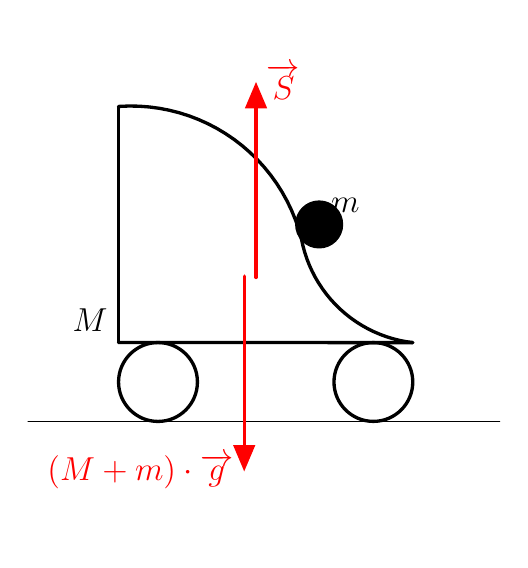
\begin{tikzpicture}[line cap=round,line join=round,>=triangle 45,x=1.0cm,y=1.0cm]
                \clip(1.,4.5) rectangle (7.,11.);
                \draw [line width=2.pt,fill=black,fill opacity=1.0] (4.701721914219811,8.501030367692636) circle (0.2703145344054361cm)
                node [anchor = south west] {$m$};
                \draw [line width=0.4pt,domain=1.:7.] plot(\x,{(--6.-0.*\x)/1.});
                \draw [line width=1.2pt] (2.65494,6.5) circle (0.5009231471595916cm);
                \draw [line width=1.2pt] (5.3903,6.5) circle (0.5003325997627946cm);
                \draw [line width=1.2pt] (2.154016852840405,7.001031293385523)node [anchor=south east] {$M$}-- (5.890632599762804,7.0002245810324295) ;
                \draw [line width=1.2pt] (2.154016852840405,9.999497321884471)-- (2.154016852840405,7.001031293385523);
                \draw [shift={(2.3120989773810603,7.773599272739968)},line width=1.2pt]  plot[domain=0.24353506308105616:1.641696766090215,variable=\t]({1.*2.231504443931177*cos(\t r)+0.*2.231504443931177*sin(\t r)},{0.*2.231504443931177*cos(\t r)+1.*2.231504443931177*sin(\t r)});
                \draw [shift={(6.077380532100785,8.618210753728665)},line width=1.2pt]  plot[domain=3.330916335599396:4.597477474744073,variable=\t]({1.*1.6287277382265966*cos(\t r)+0.*1.6287277382265966*sin(\t r)},{0.*1.6287277382265966*cos(\t r)+1.*1.6287277382265966*sin(\t r)});
                \draw [->,line width=1.2pt,color=ffqqqq] (3.75,7.8446) -- (3.75,5.36504)
                node [anchor=east] {$(M + m) \cdot \vec g$};
                \draw [->,line width=1.2pt,color=ffqqqq] (3.9,7.82794) -- (3.9,10.31)node [anchor=west] {$\vec S$};
            \end{tikzpicture}
        }
    \end{minipage}
    \begin{minipage}{.49\linewidth}
        \setlength{\parskip}{.3em}

        \begin{description}
            \item[Objet:] chariot du masse $M$ et du boulet de masse $m$ 
            \item[Forces] (externes): poids $(M+m) \vec g$ et soutien du sol $\vec S$
                \[
                    \begin{split}
                        \text{ selon } \vec{e_{x}}: &F^{\text{est}}_{x} = 0 \\
                        \implies &P_{x} = M \cdot V_{x} + m \cdot v_{x} = \text{ cste } (= 0)
                    \end{split}
                \]
                \begin{equation}
                    \implies V_{x} = - \frac{m}{M} \cdot v_{x}
                \end{equation}
        \end{description}
    \end{minipage}
\end{center}

Le chariot et le boulet ont des vitesses de signe opposé.

\paragraph{Remarques:}

\begin{itemize}
    \item Selon $\vec{e_{y}}, F^{\text{est}}_{y} \neq 0$, car le boulet descend alors
    que le chariot reste à la même hauteur.

    \item Le boulet et le chariot peuvent être pris séparément.

        \begin{center}
            \begin{minipage}{.5\linewidth}
                \resizebox{\textwidth}{!}{
                    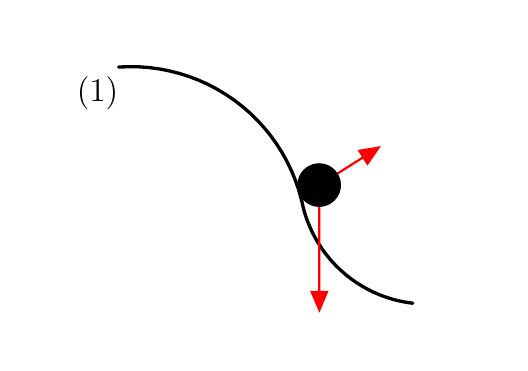
\begin{tikzpicture}[line cap=round,line join=round,>=triangle 45,x=1.0cm,y=1.0cm]
                    \clip(1.,6.5) rectangle (7.,10.5);
                    \draw (1.5, 10) node [anchor = north west] {$(1)$};
                    \draw [shift={(2.3120989773810603,7.773599272739968)},line width=1.2pt]  plot[domain=0.24353506308105616:1.641696766090215,variable=\t]({1.*2.231504443931177*cos(\t r)+0.*2.231504443931177*sin(\t r)},{0.*2.231504443931177*cos(\t r)+1.*2.231504443931177*sin(\t r)});
                    \draw [shift={(6.077380532100785,8.618210753728665)},line width=1.2pt]  plot[domain=3.330916335599396:4.597477474744073,variable=\t]({1.*1.6287277382265966*cos(\t r)+0.*1.6287277382265966*sin(\t r)},{0.*1.6287277382265966*cos(\t r)+1.*1.6287277382265966*sin(\t r)});
                    \draw [->,line width=0.8pt,color=ffqqqq] (4.701721914219811,8.501030367692636) -- (4.704317586874115,6.879720941616138);
                    \draw [->,line width=0.8pt,color=ffqqqq] (4.701721914219811,8.501030367692636) -- (5.486298039165532,8.99512377302218);
                    \draw [line width=0.4pt,fill=black,fill opacity=1.0] (4.701721914219811,8.501030367692636) circle (0.2703145344054361cm);
                    \end{tikzpicture}
                }
            \end{minipage}
            \begin{minipage}{.49\linewidth}
                \resizebox{\textwidth}{!}{
                   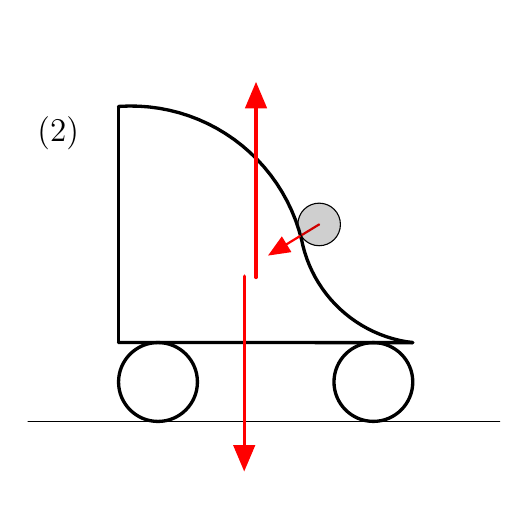
\begin{tikzpicture}[line cap=round,line join=round,>=triangle 45,x=1.0cm,y=1.0cm]
                    \clip(1.,5.) rectangle (7.,11.);
                    \draw [line width=0.4pt,domain=1.:7.] plot(\x,{(--6.-0.*\x)/1.});
                    \draw (1, 10) node [anchor = north west] {$(2)$};
                    \draw [line width=1.2pt] (2.65494,6.5) circle (0.5009231471595916cm);
                    \draw [line width=1.2pt] (5.3903,6.5) circle (0.5003325997627946cm);
                    \draw [line width=1.2pt] (2.154016852840405,7.001031293385523)-- (5.890632599762804,7.0002245810324295);
                    \draw [line width=1.2pt] (2.154016852840405,9.999497321884471)-- (2.154016852840405,7.001031293385523);
                    \draw [shift={(2.3120989773810603,7.773599272739968)},line width=1.2pt]  plot[domain=0.24353506308105616:1.641696766090215,variable=\t]({1.*2.231504443931177*cos(\t r)+0.*2.231504443931177*sin(\t r)},{0.*2.231504443931177*cos(\t r)+1.*2.231504443931177*sin(\t r)});
                    \draw [shift={(6.077380532100785,8.618210753728665)},line width=1.2pt]  plot[domain=3.330916335599396:4.597477474744073,variable=\t]({1.*1.6287277382265966*cos(\t r)+0.*1.6287277382265966*sin(\t r)},{0.*1.6287277382265966*cos(\t r)+1.*1.6287277382265966*sin(\t r)});
                    \draw [->,line width=1.2pt,color=ffqqqq] (3.75,7.8446) -- (3.75,5.36504);
                    \draw [->,line width=1.2pt,color=ffqqqq] (3.9,7.82794) -- (3.9,10.31);
                    \draw [->,line width=0.8pt,color=ffqqqq] (4.701721914219811,8.501030367692636) -- (4.052825744834581,8.105743152451883);
                    \draw [line width=0.4pt,fill=black,fill opacity=0.1899999976158142] (4.701721914219811,8.501030367692636) circle (0.2703145344054361cm);
                    \begin{scriptsize}
                    \draw[color=black] (-4.88071244979948,6.295995357097354) node {$f$};
                    \end{scriptsize}
                    \end{tikzpicture} 
                }
            \end{minipage}
        \end{center}
\end{itemize}

\begin{center}
    \begin{minipage}{.45\linewidth}
        \setlength{\parskip}{.3em}
        \begin{description}
            \item[Objet:] boulet (1)
            \item[Forces:]  poids $m \cdot \vec g$, action du chariot $\vec N$, 
                \begin{equation}
                    m \cdot \vec g + \vec N = m \cdot \vec{a_{m}}
                \end{equation}
        \end{description}
        L'accélération est dirigée le long du plan incliné vers la droite.
    \end{minipage}
    \hspace{1cm}
    \begin{minipage}{.45\linewidth}
        \setlength{\parskip}{.3em}
        \begin{description}
            \item[Objet:] chariot (2)
            \item[Forces:]  poids $M \cdot \vec g$, soutien du sol $\vec S$, réaction du chariot $\vec N$, 
                \begin{equation}
                    M \cdot \vec g + \vec S - \vec N = M \cdot \vec{a_{M}}
                \end{equation}
        \end{description}
        L'accélération est dirigée vers la gauche.\\
    \end{minipage}
\end{center}

\subsection{Blocs superposés}

On considère un objet constitué de deux blocs superposés. L'un est tracté et
glisse sans frottements sur le sol. L'autre bloc est posé sur le premier. Les
deux blocs sont immobiles l'un par rapport à l'autre; leur accélération $\vec a$
est identique.

\begin{center}
    \begin{minipage}{.5\linewidth}
        \resizebox{\textwidth}{!}{
            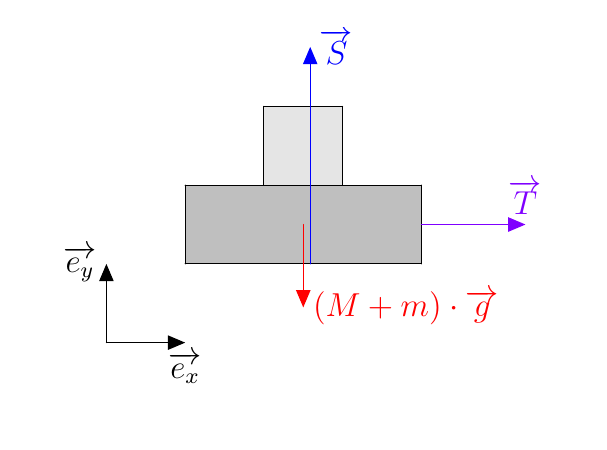
\begin{tikzpicture}[line cap=round,line join=round,>=triangle 45,x=1.0cm,y=1.0cm]
            \clip(0,0) rectangle (7.,5.);
            \fill[line width=0.4pt,fill=black,fill opacity=0.25] (2.,3.) -- (2.,2.) -- (5.,2.) -- (5.,3.) -- cycle;
            \fill[line width=0.4pt,fill=black,fill opacity=0.10000000149011612] (3.,4.) -- (3.,3.) -- (4.,3.) -- (4.,4.) -- cycle;
            \draw [->,line width=0.4pt, shift={(1, 1)}] (0.,0.) -- (0.,1.) node [anchor = east]{$\vec{e_y}$};
            \draw [->,line width=0.4pt, shift={(1, 1)}] (0.,0.) -- (1.,0.) node [anchor = north]{$\vec{e_x}$};
            \draw [line width=0.4pt] (2.,3.)-- (2.,2.);
            \draw [line width=0.4pt] (2.,2.)-- (5.,2.);
            \draw [line width=0.4pt] (5.,2.)-- (5.,3.);
            \draw [line width=0.4pt] (5.,3.)-- (2.,3.);
            \draw [line width=0.4pt] (3.,4.)-- (3.,3.);
            \draw [line width=0.4pt] (3.,3.)-- (4.,3.);
            \draw [line width=0.4pt] (4.,3.)-- (4.,4.);
            \draw [line width=0.4pt] (4.,4.)-- (3.,4.);
            \draw [->,line width=0.4pt,color=ffqqqq] (3.5,2.5) -- (3.5,1.4476289196110619) node [anchor=west]{$(M+m) \cdot \vec g$};
            \draw [->,line width=0.4pt,color=qqqqff] (3.5882171110761467,2.) -- (3.5882171110761467,4.755379216198521)
            node [anchor = west] {$\vec S$};
            \draw [->,line width=0.4pt,color=xfqqff] (5.,2.5) -- (6.32170520339495,2.5)
            node [anchor = south] {$\vec T$};
            \end{tikzpicture}
        }
    \end{minipage}
    \begin{minipage}{.49\linewidth}
        \setlength{\parskip}{.3em}

        \begin{description}
            \item[Objet:] les deux blocs
            \item[Forces:] Poids $(M+m)\cdot \vec g$, soutien $\vec S$, traction $\vec T$
                $$\vec T + (M+m)\cdot \vec g + \vec S = (M+m) \cdot \vec a$$
                \begin{equation}
                    \label{eq:3.28}
                    \text{ selon } \vec{e_{x}}: \quad T = (M+m) \cdot a
                \end{equation}
        \end{description}
    \end{minipage}
\end{center}

\begin{center}
    \begin{minipage}{.5\linewidth}
        \resizebox{\textwidth}{!}{
            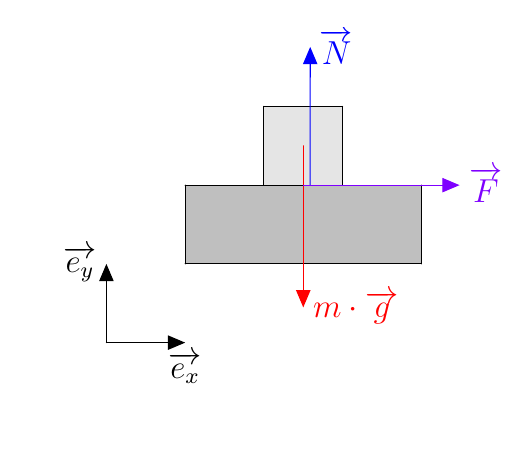
\begin{tikzpicture}[line cap=round,line join=round,>=triangle 45,x=1.0cm,y=1.0cm]
            \clip(0.,0.) rectangle (6.,5.);
            \fill[line width=0.4pt,fill=black,fill opacity=0.25] (2.,3.) -- (2.,2.) -- (5.,2.) -- (5.,3.) -- cycle;
            \fill[line width=0.4pt,fill=black,fill opacity=0.10000000149011612] (3.,4.) -- (3.,3.) -- (4.,3.) -- (4.,4.) -- cycle;
            \draw [->,line width=0.4pt, shift={(1, 1)}] (0.,0.) -- (0.,1.) node [anchor = east]{$\vec{e_y}$};
            \draw [->,line width=0.4pt, shift={(1, 1)}] (0.,0.) -- (1.,0.) node [anchor = north]{$\vec{e_x}$};
            \draw [line width=0.4pt] (2.,3.)-- (2.,2.);
            \draw [line width=0.4pt] (2.,2.)-- (5.,2.);
            \draw [line width=0.4pt] (5.,2.)-- (5.,3.);
            \draw [line width=0.4pt] (5.,3.)-- (2.,3.);
            \draw [line width=0.4pt] (3.,4.)-- (3.,3.);
            \draw [line width=0.4pt] (3.,3.)-- (4.,3.);
            \draw [line width=0.4pt] (4.,3.)-- (4.,4.);
            \draw [line width=0.4pt] (4.,4.)-- (3.,4.);
            \draw [->,line width=0.4pt,color=qqqqff] (3.5871549029320566,3.) -- (3.5882171110761467,4.755379216198521) node [anchor=west]{$\vec N$};
            \draw [->,line width=0.4pt,color=ffqqqq] (3.5,3.5) -- (3.5,1.4476289196110619) node [anchor=west]{$m \cdot \vec g$};
            \draw [->,line width=0.4pt,color=xfqqff] (3.501393236048519,3.) -- (5.484745350227967,3.) node [anchor=west]{$\vec F$};
            \begin{scriptsize}
            \end{scriptsize}
            \end{tikzpicture}
        }
    \end{minipage}
    \begin{minipage}{.49\linewidth}
        \setlength{\parskip}{.3em}
        \begin{description}
            \item[Objet:] le bloc supérieur
            \item[Forces:] Poids $m\cdot \vec g$, soutien du bloc inférieur $\vec N$, frottement $\vec F$
                $$\vec F + m \cdot \vec g + \vec N = m \cdot \vec a$$
                \begin{equation}
                    \label{eq:3.29}
                    \text{ selon } \vec{e_{x}}: \quad F = m \cdot a
                \end{equation}
        \end{description}
    \end{minipage}
\end{center}

A l'aide des équations du mouvement $\eqref{eq:3.28}$ et $\eqref{eq:3.29}$
$$
\left\{
    \begin{array}{lc}
        T = (M+m) \cdot a & \eqref{eq:3.28}\\
        F = m \cdot a& \eqref{eq:3.29}\\
    \end{array}
\right.
$$
On fixe l'expression de la norme $F$ de la force du frottement 

\begin{equation}
    \label{eq:3.30}
    f=  \frac{m}{m+M} \cdot T
\end{equation}

\paragraph{Remarque:}

En considérant comme objet le bloc inférieur, on aurait obtenu la loi du
mouvement suivante:
$$\vec T + M \vec g + \vec S- \vec F - \vec N = M\cdot \vec a$$
où les signes négatifs sont le résultat de la $2^{e}$ loi de Newton 
\begin{equation}
    \label{eq:3.31}
    \text{ selon } \vec{e_{x}}: T - F = m \cdot a 
\end{equation}

Les équations du mouvement $\eqref{eq:3.28}, \eqref{eq:3.29}$ et $\eqref{eq:3.31}$
sont linéairement dépendantes


\section{Pression}
\label{sec:pression}

On considère une force $\vec F$ exercée sur la surface $S$ d'un objet:

\begin{center}
    \begin{minipage}{.5\linewidth}
        \resizebox{\textwidth}{!}{
            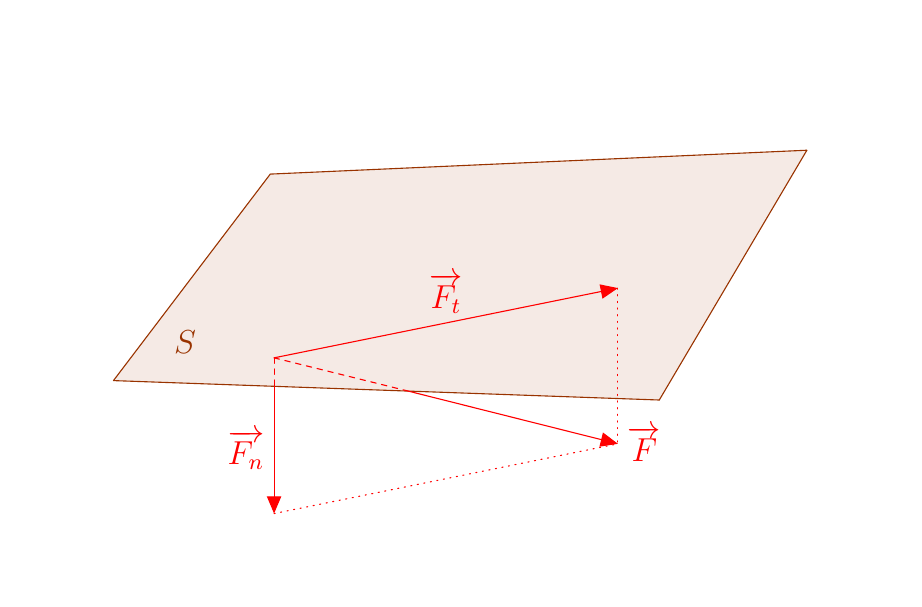
\begin{tikzpicture}[line cap=round,line join=round,>=triangle 45,x=1.0cm,y=1.0cm]
                \clip(0.,0.) rectangle (11.,7.);
                \fill[line width=0.4pt,color=zzttqq,fill=zzttqq,fill opacity=0.10000000149011612] (3.0809148186930804,5.140286431107078) -- (1.0894074216255951,2.517806393384548) -- (8.021410465070378,2.271246852437896) -- (9.895906263100072,5.443470510641992) -- cycle;
                \draw [line width=0.4pt,color=zzttqq] (3.0809148186930804,5.140286431107078)-- (1.0894074216255951,2.517806393384548);
                \draw [line width=0.4pt,color=zzttqq] (1.0894074216255951,2.517806393384548)-- (8.021410465070378,2.271246852437896);
                \draw [line width=0.4pt,color=zzttqq] (8.021410465070378,2.271246852437896)-- (9.895906263100072,5.443470510641992);
                \draw [line width=0.4pt,color=zzttqq] (9.895906263100072,5.443470510641992)-- (3.0809148186930804,5.140286431107078);
                \draw [->,line width=0.4pt,color=ffqqqq] (3.129182420762114,2.80681708044638) -- (7.496139664523596,3.6925678421527186) node [anchor= south, midway]{$\vec{F_t}$};
                \draw [->,line width=0.4pt,color=ffqqqq] (3.129182420762114,2.445255071022226) -- (3.129182420762114,0.8293270077996704) node [anchor = east, midway]{$\vec{F_n}$};
                \draw [line width=0.4pt,dash pattern=on 2pt off 2pt,color=ffqqqq] (3.129182420762114,2.80681708044638)-- (3.129182420762114,2.445255071022226);
                \draw [line width=0.4pt,dotted,color=ffqqqq] (3.129182420762114,0.8293270077996704)-- (7.496139664523596,1.715077769506009);
                \draw [line width=0.4pt,dotted,color=ffqqqq] (7.496139664523596,3.6925678421527186)-- (7.496139664523596,1.715077769506009);
                \draw [line width=0.4pt,dash pattern=on 2pt off 2pt,color=ffqqqq] (3.129182420762114,2.80681708044638)-- (4.8317073063178,2.384699160760499);
                \draw [->,line width=0.4pt,color=ffqqqq] (4.8317073063178,2.384699160760499) -- (7.496139664523596,1.715077769506009) node [anchor = west]{$\vec{F}$};
                \begin{scriptsize}
                \draw[color=zzttqq] (2,3) node {$S$};
                \end{scriptsize}
            \end{tikzpicture}
        }
    \end{minipage}
    \begin{minipage}{.49\linewidth}
        \setlength{\parskip}{.3em}
        On décompose la force $\vec F$:
        \begin{equation}
            \vec F = \vec{F_{n}} + \vec{F_{t}}
        \end{equation}
        où \begin{itemize}
            \item $\vec{F_{n}}=$ force normale, de compression
            \item $\vec{F_{t}}=$ force tangente, de cisaillement
        \end{itemize}
    \end{minipage}
\end{center}

\subsection{Pression moyenne}
\label{sub:pression_moyenne}

\begin{itemize}
    \item La pression moyenne est définie comme le rapport de la norme de la
        force normale et de la surface.
        \begin{equation}
            p_{moy} = \frac{\| \vec{F_{n}}\|}{S}
        \end{equation}
    \item Elle nous donne la répartition moyenne de la force normale sur la
        surface de l'objet.
    \item Unité physique de la pression (SI): Pascale [$Pa$] = $\left[\frac{N}{m^{2}}\right]$
        = $\left[\frac{kg}{m \cdot s^{2}}\right]$
\end{itemize}

\paragraph{Exemple:}

Une personne de masse $m = 64 kg$ se tient sur un talon. On calcule la
pression moyenne exercée sur le pieds du voisin.
\begin{itemize}
    \item À l'équilibre, la force exercée sur le sol est le poids de la
        personne $m \cdot \vec g$. Ainis,
        \begin{equation}
            p_{moy} = \frac{m\cdot g}{S}
        \end{equation}
    \item Talon plat: $$S = 16 cm^{2} \implies p_{moy} = \frac{640 N }{16\cdot
        10^{-4} m^{2}} = 4 \cdot 10^{5}Pa$$
    \item Talon plat: $$S = 1 cm^{2} \implies p_{moy} = \frac{640 N }{1\cdot
        10^{-4} m^{2}} = 64 \cdot 10^{5}Pa$$
\end{itemize}

Pour exercer la même pression sur le sol avec un talon plat qu'avec un talon
aiguille, il faudrait que la personne porte  15 autre personnes de masse
identiques.

\subsection{Pression locale}
\label{sub:pression_locale}

La force normale $\vec{F_{n}}$ n'agit à priori pas de la même manière sur
toute la surface d'air $S$. En divisant la surface en éléments d'air $\Delta S$, 
on met en évidence la contribution de $\Delta \vec{F_{n}}$ sur chaque $\Delta
S$.

\begin{center}
    \begin{minipage}{.5\linewidth}
        \resizebox{\textwidth}{!}{
            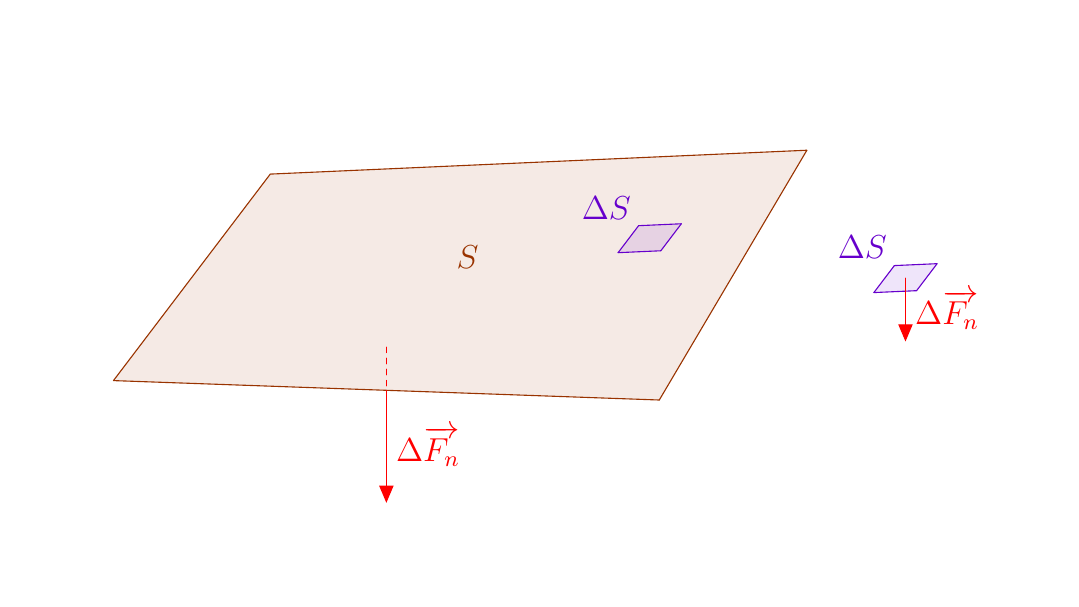
\begin{tikzpicture}[line cap=round,line join=round,>=triangle 45,x=1.0cm,y=1.0cm]
            \clip(0.,0.) rectangle (13.,7.);
            \fill[line width=0.4pt,color=zzttqq,fill=zzttqq,fill opacity=0.10000000149011612] (3.0809148186930804,5.140286431107078) -- (1.0894074216255951,2.517806393384548) -- (8.021410465070378,2.271246852437896) -- (9.895906263100072,5.443470510641992) -- cycle;
            \fill[line width=0.4pt,color=wwqqcc,fill=wwqqcc,fill opacity=0.10000000149011612] (7.758728949426308,4.485220757715192) -- (7.498405592338266,4.14241871323292) -- (8.04097479148095,4.166556431463083) -- (8.301298148568993,4.509358475945356) -- cycle;
            \fill[line width=0.4pt,color=wwqqcc,fill=wwqqcc,fill opacity=0.10000000149011612] (11.00690413258813,3.978457879714531) -- (10.746580775500089,3.6356558352322597) -- (11.289149974642774,3.659793553462423) -- (11.549473331730814,4.002595597944695) -- cycle;
            \draw [line width=0.4pt,color=zzttqq] (3.0809148186930804,5.140286431107078)-- (1.0894074216255951,2.517806393384548);
            \draw [line width=0.4pt,color=zzttqq] (1.0894074216255951,2.517806393384548)-- (8.021410465070378,2.271246852437896);
            \draw [line width=0.4pt,color=zzttqq] (8.021410465070378,2.271246852437896)-- (9.895906263100072,5.443470510641992);
            \draw [line width=0.4pt,color=zzttqq] (9.895906263100072,5.443470510641992)-- (3.0809148186930804,5.140286431107078);
            \draw [->,line width=0.4pt,color=ffqqqq] (4.555388568975854,2.394527347592935) -- (4.555388568975854,0.9653816129997463) node [anchor = west, midway] {$\Delta \vec{F_n}$};
            \draw [line width=0.4pt,dash pattern=on 2pt off 2pt,color=ffqqqq] (4.555388568975854,2.942871685646456)-- (4.555388568975854,2.394527347592935);
            \draw [line width=0.4pt,color=wwqqcc] (7.758728949426308,4.485220757715192)-- (7.498405592338266,4.14241871323292);
            \draw [line width=0.4pt,color=wwqqcc] (7.498405592338266,4.14241871323292)-- (8.04097479148095,4.166556431463083);
            \draw [line width=0.4pt,color=wwqqcc] (8.04097479148095,4.166556431463083)-- (8.301298148568993,4.509358475945356);
            \draw [line width=0.4pt,color=wwqqcc] (8.301298148568993,4.509358475945356)-- (7.758728949426308,4.485220757715192);
            \draw [line width=0.4pt,color=wwqqcc] (11.00690413258813,3.978457879714531)-- (10.746580775500089,3.6356558352322597);
            \draw [line width=0.4pt,color=wwqqcc] (10.746580775500089,3.6356558352322597)-- (11.289149974642774,3.659793553462423);
            \draw [line width=0.4pt,color=wwqqcc] (11.289149974642774,3.659793553462423)-- (11.549473331730814,4.002595597944695);
            \draw [line width=0.4pt,color=wwqqcc] (11.549473331730814,4.002595597944695)-- (11.00690413258813,3.978457879714531);
            \draw [->,line width=0.4pt,color=ffqqqq] (11.14802705361545,3.819125716588477) -- (11.14802705361545,3.0140570274342426) node [anchor = west, midway] {$\Delta \vec{F_n}$};
            \begin{scriptsize}
            \draw[color=zzttqq] (5.588236305220915,4.081304952603675) node {$S$};
            \draw[color=wwqqcc] (7.75,4.48) node [anchor = south east]{$\Delta S$};
            \draw[color=wwqqcc] (11,3.978) node [anchor = south east]{$\Delta S$};
            \end{scriptsize}
            \end{tikzpicture}
        }
    \end{minipage}
    \begin{minipage}{.49\linewidth}
        \setlength{\parskip}{.3em}
        \begin{description}
            \item[Surface totale:] $S = \Delta S_{1} + \Delta S_{2} + ...$
            \item[Force normale:] $F_{n} = \Delta F_{n,1} + \Delta F_{n,2} + ...$
            \item[Pression locale:] $$p(\vec r) = \lim_{\Delta S \to 0} \frac{\|
                \Delta \vec{F_{n}}}{\Delta S} = \frac{dF_{n}}{dS}$$
        \end{description}
    \end{minipage}
\end{center}

\paragraph{Remarque:}

La pression est

\begin{enumerate}
    \item Un scalaire positif, $p \geq 0$
    \item Définie en tout point $\vec r$ de la surface, à priori différente d'un
        à un autre: c'est une fonction de l'espace (et du temps)
        $$p \equiv p (\vec r, t)$$
\end{enumerate}


\paragraph{Cas particuliers}

Si la force normale est uniforme sur la surface $S$, alors la pression est
identique en tout point et est égale à la pression moyenne. Ainsi
\begin{equation}
    \| \vec{F_{n}} \| = p \cdot S 
\end{equation}

\paragraph{Exemple:}

La pression de l'air due aux chocs des molécules d'aires sur les faces.

\subsection{Gaz dans un cylindre}
\label{sub:gaz_dans_un_cylindre}

\begin{center}
    \begin{minipage}{.5\linewidth}
        \resizebox{\textwidth}{!}{
            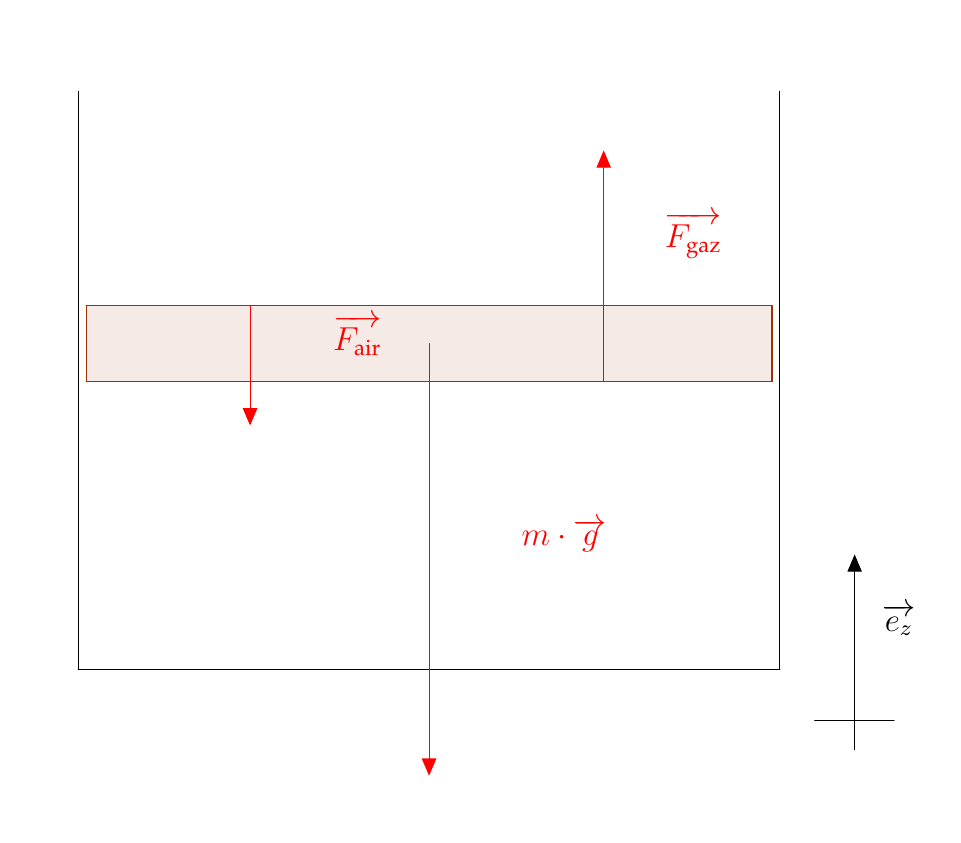
\begin{tikzpicture}[line cap=round,line join=round,>=triangle 45,x=1.0cm,y=1.0cm]
            \clip(3.,1.) rectangle (14.5,11.);
            \fill[line width=0.4pt,color=zzttqq,fill=zzttqq,fill opacity=0.10000000149011612] (3.7419043656825894,7.469321270984043) -- (3.7419043656825894,6.505089500197211) -- (12.453331165465356,6.505089500197211) -- (12.453331165465356,7.469321270984043) -- cycle;
            \draw [line width=0.4pt] (3.6419043656825894,10.192062646125509)-- (3.6419043656825894,2.846532986517624);
            \draw [line width=0.4pt] (12.553331165465355,2.846532986517624)-- (3.6419043656825894,2.846532986517624);
            \draw [line width=0.4pt] (12.553331165465355,2.846532986517624)-- (12.553331165465355,10.192062646125509);
            \draw [line width=0.4pt,color=zzttqq] (3.7419043656825894,7.469321270984043)-- (3.7419043656825894,6.505089500197211);
            \draw [line width=0.4pt,color=zzttqq] (3.7419043656825894,6.505089500197211)-- (12.453331165465356,6.505089500197211);
            \draw [line width=0.4pt,color=zzttqq] (12.453331165465356,6.505089500197211)-- (12.453331165465356,7.469321270984043);
            \draw [line width=0.4pt,color=zzttqq] (12.453331165465356,7.469321270984043)-- (3.7419043656825894,7.469321270984043);
            \draw [->,line width=0.4pt,color=ffqqqq] (8.097617765573972,6.987205385590629) -- (8.097617765573972,1.499548182887108);
            \draw [->,line width=0.4pt,color=ffqqqq] (5.824247674766614,7.469321270984043) -- (5.824247674766614,5.947778715995135);
            \draw [->,line width=0.4pt,color=ffqqqq] (10.315572261122268,6.505089500197211) -- (10.315572261122268,9.440805256149606);
            \draw [line width=0.4pt] (12.995952568933559,2.2023789387431743)-- (14.002355615766017,2.2023789387431743);
            \draw [->,line width=0.4pt] (13.502486552769764,1.83235066947432) -- (13.502486552769764,4.309699658398218);
            \begin{scriptsize}
            \draw[color=ffqqqq] (9.81631973210362,4.549656712550469) node {$m \cdot \vec g$};
            \draw[color=ffqqqq] (7.187642591024057,7.0929871932053725) node {$\vec{F_{\text{air}}}$};
            \draw[color=ffqqqq] (11.454975612257115,8.356117767490359) node {$\vec{F_{\text{gaz}}}$};
            \draw[color=black] (14.066583421251748,3.474288791199739) node {$\vec{e_z}$};
            \end{scriptsize}
            \end{tikzpicture}
        }
    \end{minipage}
    \begin{minipage}{.49\linewidth}
        \setlength{\parskip}{.3em}
        \begin{description}
            \item[Objet:] piston
            \item[Forces:] poids $m \cdot \vec g$ et forces de pression $\vec{F_{\text{air}}}$
                et $\vec{F_{\text{gaz}}}$
                $$m \cdot \vec g + \vec{F_{\text{air}}} + \vec{F_{\text{gaz}}}
                = \vec 0 \quad \text{ (à l'équilibre) }$$
                $$\text{ selon } \vec{e_{x}}: -m \cdot g - p_{\text{air}}\cdot S+ p_{\text{air}}\cdot S = 0
                \implies$$
                $$p_{\text{gaz}} = p_{\text{air}} + \frac{m\cdot g}{S}$$
        \end{description}
    \end{minipage}
\end{center}

\paragraph{Remarque:}
La pression de l'air à la surface de la terre a, en général, une valeur
comprise entre 
$$0.95 \cdot 10^{5}Pa < p_{\text{air}} < 1.05 \cdot 10 ^{5}Pa$$

\paragraph{Autres unités de pression:}

\begin{description}
\item[Bar:] $1 bar = 10^{5}Pa$
\item[Atmosphère] $1 atm = 1.013 \cdot 10^{5}Pa$
\item[Millimètre de mercure] $1 atm = 760 mmMg$
\end{description}


\subsection{Loi des gaz parfaits}
\label{sub:loi_des_gaz_parfaits}

Un gaz parfait est un modèle de gaz idéalisé. Lorsque la pression d'un gaz est
suffisamment basse, les gaz réels peuvent être modélisé par les modèles de gaz
parfait.. Dans le cas contraire, ils sont décrit par le mode du gaze de Van
der Waals.


\begin{highlightBox}[frametitle={Équations d'était du gaz parfait}]
\begin{equation}
    p \cdot V = N \cdot k \cdot T = n \cdot R \cdot T
\end{equation}
\end{highlightBox}
où 
\begin{itemize}
    \item $p$ est la pression du gaz [$Pa$]
    \item $V$ est le volume occupé par le gaz [$m^{3}$]
    \item $T$ la température du gaz [$K$]
    \item $k$ est la constante de Boltzmann: $x = 1.38 \cdot 10^{-23}
        \left[\frac{J}{K}\right]$
    \item $N_{A}$ est le nombre d'Avogadro: $N_{A} = 6.02 \cdot 10 ^{23}
        \text{ molécules } $
    \item $n$ est le nombre de moles de gaz: $n = \frac{N}{N_{A}}$
    \item $R$ est la constante de gaz parfait: $R = N_{A} \cdot k = 8.31
        \left[\frac{J}{K\cdot mol}\right]$
\end{itemize}

\section{Hydrostatique}


\subsection{Définition d'un fluide}
\label{sub:definition_d_un_fluide}

\begin{center}
    \begin{minipage}{.5\linewidth}
        \resizebox{\textwidth}{!}{
            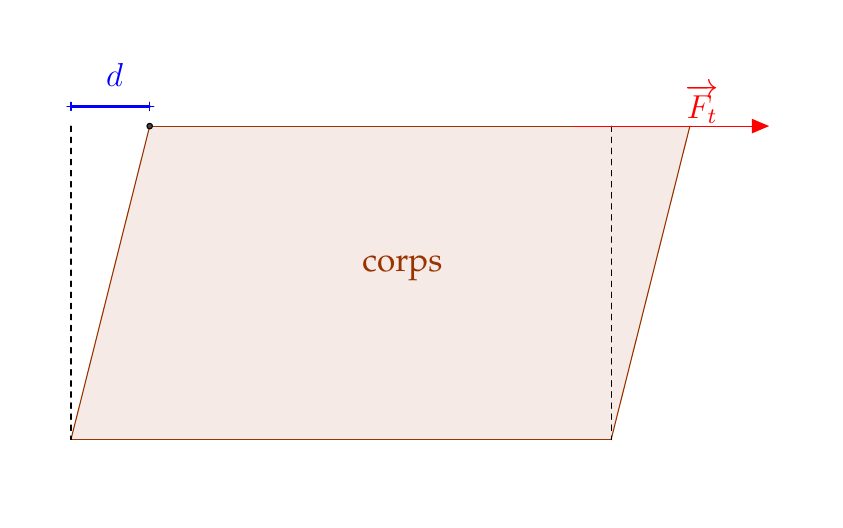
\begin{tikzpicture}[line cap=round,line join=round,>=triangle 45,x=1.0cm,y=1.0cm]
            \clip(-10.,1.) rectangle (0.,7.);
            \fill[line width=0.4pt,color=zzttqq,fill=zzttqq,fill opacity=0.10000000149011612] (-8.45,5.75) -- (-9.45,1.77) -- (-2.59,1.77) -- (-1.59,5.75) -- cycle;
            \draw [line width=0.4pt,color=zzttqq] (-8.45,5.75)-- (-9.45,1.77);
            \draw [line width=0.4pt,color=zzttqq] (-9.45,1.77)-- (-2.59,1.77);
            \draw [line width=0.4pt,color=zzttqq] (-2.59,1.77)-- (-1.59,5.75);
            \draw [line width=0.4pt,color=zzttqq] (-1.59,5.75)-- (-8.45,5.75);
            \draw [line width=0.4pt,dash pattern=on 2pt off 2pt] (-9.45,5.75)-- (-9.45,1.77);
            \draw [line width=0.4pt,dash pattern=on 2pt off 2pt] (-2.59,5.75)-- (-2.59,1.77);
            \draw [line width=0.8pt,color=qqqqff] (-9.45,6.)-- (-8.45,6.);
            \draw [->,line width=0.4pt,color=ffqqqq] (-3.058260119842952,5.75) -- (-0.5835200332905446,5.75);
            \begin{scriptsize}
            \draw [fill=uuuuuu] (-8.45,5.75) circle (1.0pt);
            \draw[color=zzttqq] (-5.239963973646891,3.937930517545855) node {corps};
            \draw [color=qqqqff] (-9.45,6.)-- ++(-1.5pt,0 pt) -- ++(3.0pt,0 pt) ++(-1.5pt,-1.5pt) -- ++(0 pt,3.0pt);
            \draw [color=qqqqff] (-8.45,6.)-- ++(-1.5pt,0 pt) -- ++(3.0pt,0 pt) ++(-1.5pt,-1.5pt) -- ++(0 pt,3.0pt);
            \draw[color=qqqqff] (-8.897152377339697,6.395718423253387) node {$d$};
            \draw[color=ffqqqq] (-1.4353082956116312,6.0319658132086715) node {$\vec{F_t}$};
            \end{scriptsize}
            \end{tikzpicture}
        }
    \end{minipage}
    \begin{minipage}{.49\linewidth}
        \setlength{\parskip}{.3em}
        Si on applique une force tangentielle de cisaillement $\vec{F_{t}}$
        pour obtenir un petit déplacement tangentiel $d$, le corps s'oppose à
        ce cisaillement.
    \end{minipage}
\end{center}
\begin{itemize}
    \item Le corps est \textbf{solide} s'il faut exercer une force de cisaillement en
        continu pour maintenir un déplacement.

        \paragraph{Exemple:}

        Modèle linéaire $$F_{t} = k \cdot d \quad \text{(force élastique)}$$
        En régime élastique, le solide reprend sa forme initiale si on supprime la
        force de cisaillement.

    \item Le corps est un \textbf{fluide}, si la force de cisaillement
        nécessaire pour maintenir le déplacement diminue au cours du temps.
        Après un temps suffisamment grand, plus aucun cisaillement n'est
        nécessaire, le fluide s'est adapté à la contrainte.

        \paragraph{Exemple:}
        
        Modèle exponentiel $$F_{t} = k \cdot d \cdot e^{-\lambda \cdot t}$$
        Si on maintient ce cisaillement (même très faible), le fluide se
        transforme continuellement.
\end{itemize}

\subsection{Forces dans un fluide au repos}

L'hydrostatique est l'étude des fluides au repos.

\begin{center}
    \begin{minipage}{.5\linewidth}
        \resizebox{\textwidth}{!}{
            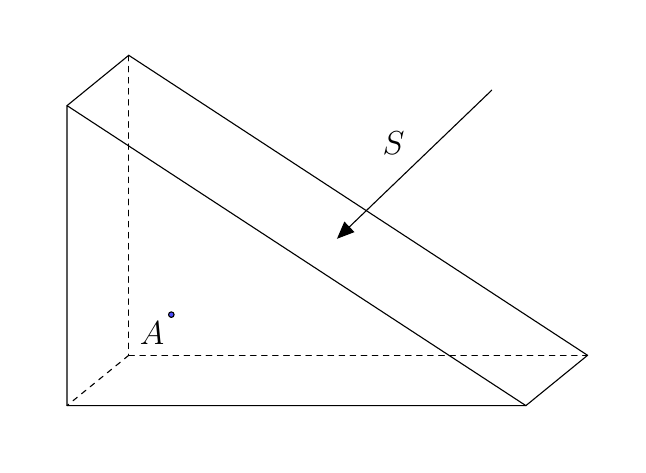
\begin{tikzpicture}[line cap=round,line join=round,>=triangle 45,x=1.0cm,y=1.0cm]
            \clip(2.,3.) rectangle (9.5,8.3);
            \draw[line width=0.4pt] (2.5,7.31002) -- (2.5,3.5) -- (8.32703,3.5) -- cycle;
            \draw [line width=0.4pt,dash pattern=on 2pt off 2pt] (3.2836444833468343,7.949040379660555)-- (3.2836444833468343,4.139020379660548);
            \draw [line width=0.4pt,dash pattern=on 2pt off 2pt] (3.2836444833468343,4.139020379660548)-- (9.110674483346848,4.139020379660548);
            \draw [line width=0.4pt] (9.110674483346848,4.139020379660548)-- (3.2836444833468343,7.949040379660555);
            \draw [line width=0.4pt] (2.5,7.31002)-- (3.2836444833468343,7.949040379660555);
            \draw [line width=0.4pt,dash pattern=on 2pt off 2pt] (3.2836444833468343,4.139020379660548)-- (2.5,3.5);
            \draw [line width=0.4pt] (8.32703,3.5)-- (9.110674483346848,4.139020379660548);
            \draw [->,line width=0.4pt,color=black] (7.894454594454163,7.506638556633193) -- (5.928224269888137,5.619057445049808) node [anchor = south east, midway] {$S$};
            \begin{scriptsize}
            \draw [fill=ududff] (3.8243578226024906,4.655604586012456) circle (1.0pt) node [anchor=north east]{$A$};
            \end{scriptsize}
            \end{tikzpicture}
        }
    \end{minipage}
    \begin{minipage}{.49\linewidth}
        \setlength{\parskip}{.3em}
        Dans un fluide, on considère un petit volume autour du point $A$.
    \end{minipage}
\end{center}
En coupe,

\begin{center}
    \begin{minipage}{.5\linewidth}
        \resizebox{\textwidth}{!}{
            \begin{tikzpicture}[line cap=round,line join=round,>=triangle 45,x=1.0cm,y=1.0cm]
            \clip(2.,1.5) rectangle (9.25,8.);
            \draw [line width=0.4pt] (2.5,7.31002) -- (2.5,3.5) -- (8.32703,3.5) -- cycle;
            \draw [line width=0.4pt] (2.5,7.31002)-- (2.5,3.5);
            \draw [line width=0.4pt] (2.5,3.5)-- (8.32703,3.5);
            \draw [line width=0.4pt] (8.32703,3.5)-- (2.5,7.31002);
            \draw [->,line width=0.4pt,color=black] (7.566436732507534,7.202050541968466) -- (5.600206407941508,5.314469430385082) node [anchor=south east, midway]{$S$};
            \draw [->,line width=0.4pt,color=qqqqff] (4.609534536321321,5.9306948937151605) -- (8.734559262214802,3.2335358425092036) node [anchor=south west, midway]{$\vec{F_{t}}$};
            \draw [->,line width=0.4pt,color=qqqqff] (4.609534536321321,5.9306948937151605) -- (3.7318935960140727,4.588434199965903) node [anchor=east, midway]{$\vec{F_{n}}$};
            \draw [->,line width=0.4pt,color=qqqqff] (4.609534536321321,5.9306948937151605) -- (7.856918321907553,1.891275148759946) node [anchor=south, midway]{$\vec F$};
            \begin{scriptsize}
            \draw [fill=ududff] (3.1417953104454486,4.666525144135185) circle (1.0pt) node [anchor=north east]{$A$};
            \end{scriptsize}
            \end{tikzpicture} 
        }
    \end{minipage}
    \begin{minipage}{.49\linewidth}
        \setlength{\parskip}{.3em}
        Le fluide environnant exercent une force $\vec F$ sur chaque face de
        surface $S$: 
        \begin{equation}
            \vec F = \vec{F_{t}} + \vec{F_{n}}
        \end{equation}
        Comme le fluide est au repos il n'exerce pas réellement de
        cisaillement ( sinon il se déforment ): $$\vec{F_{t}} = \vec 0$$. Ainsi
        la force $\vec F$ est normale à la face $$\vec F = \vec{F_{n}}$$
    \end{minipage}
\end{center}


\subsection{Loi de Pascal}

L'intensité de la force exercée par le fluide sur la surface ne dépend pas de
l'orientation de la surface. Elle dépend de la taille de la surface et de sa
position $\vec r$ dans le fluide. Il suffit de conna\^itre la pression (force
par unité de surface) de fluide $p(\vec r)$.

\paragraph{Remarque:}

Lors de chocs sur une surface, les molécules changent de quantité de mouvement
et subissent une force de la part de la surface. La $3^{e}$ loi de Newton
implique que les molécules exercent une force, nommée de pression.

\subsection{Loi d'hydrostatique}
\label{sub:loi_d_hydrostatique}

On considère un fluide au repos, soummis à la force de la gravité. Par
experience, la pression augmente avec la profondeur (oreilles).

\begin{center}
    \begin{minipage}{.5\linewidth}
        \resizebox{\textwidth}{!}{
            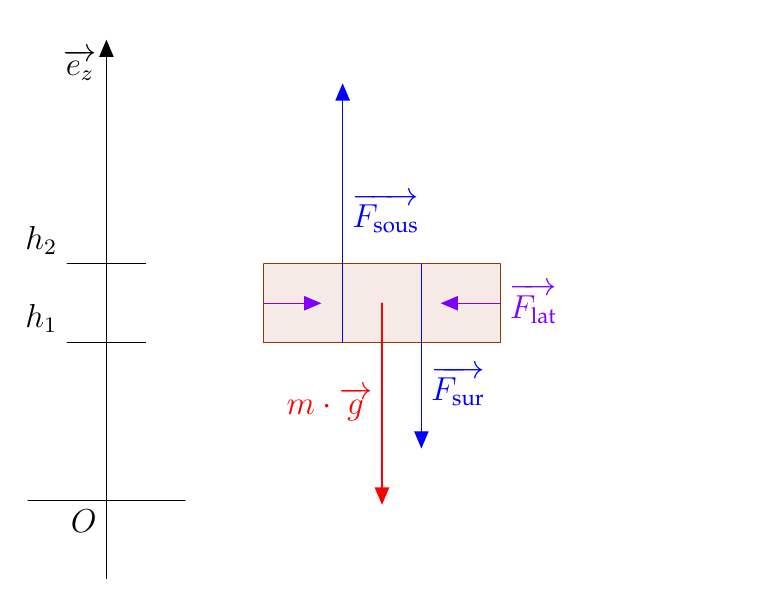
\begin{tikzpicture}[line cap=round,line join=round,>=triangle 45,x=1.0cm,y=1.0cm]
            \clip(1.,1.) rectangle (10.,8.);
            \fill[line width=0.4pt,color=zzttqq,fill=zzttqq,fill opacity=0.10000000149011612] (4.,5.) -- (4.,4.) -- (7.,4.) -- (7.,5.) -- cycle;
            \draw [line width=0.4pt] (1.,2.)-- (3.,2.);
            \draw (2, 2) node [anchor=north east] {$O$};
            \draw [->,line width=0.4pt] (2.,1.) -- (2.,7.846827418527504)
            node[anchor = north east] {$\vec{e_{z}}$};
            \draw [line width=0.4pt] (1.50036389959032,5.) node [anchor = south east] {$h_{2}$}-- (2.4971588856213867,5.);
            \draw [line width=0.4pt] (1.50036389959032,4.) node [anchor = south east] {$h_{1}$}-- (2.4971588856213867,4.);
            \draw [line width=0.4pt,color=zzttqq] (4.,5.)-- (4.,4.);
            \draw [line width=0.4pt,color=zzttqq] (4.,4.)-- (7.,4.);
            \draw [line width=0.4pt,color=zzttqq] (7.,4.)-- (7.,5.);
            \draw [line width=0.4pt,color=zzttqq] (7.,5.)-- (4.,5.);
            \draw [->,line width=0.4pt,color=ffqqqq] (5.5,4.5) -- (5.5,1.9413074537483528) node [anchor=east, midway]{$m \cdot \vec g$};
            \draw [->,line width=0.4pt,color=qqqqff] (5.,4.) -- (5.,7.293482478865902) node [anchor = west, midway]{$\vec{F_{\text{sous}}}$};
            \draw [->,line width=0.4pt,color=qqqqff] (6.,5.) -- (6.,2.6553190973790546) node [anchor = north west, midway]{$\vec{F_{\text{sur}}}$};
            \draw [->,line width=0.4pt,color=xfqqff] (4.,4.5) -- (4.72970767418272,4.5);
            \draw [->,line width=0.4pt,color=xfqqff] (7.,4.5) node [anchor = west] {$\vec{F_{\text{lat}}}$} -- (6.245239377820354,4.5);
            \end{tikzpicture}
        }
    \end{minipage}
    \begin{minipage}{.49\linewidth}
        \setlength{\parskip}{.3em}
        \begin{description}
            \item[Objet:] parallélépipède rectangle de fluide entre deux
                niveaux $h_{1}$ et $h_{2}$
            \item[Forces] poids $m\cdot \vec g$ et forces de pression
                verticale $\vec{F_{\text{sur}}}$ et $\vec{F_{\text{sous}}}$
                et latérales $\vec{F_{\text{lat}}}$
                $$m \cdot \vec g + \vec{F_{\text{sous}}}+ \vec{F_{\text{sur}}}+ \vec{F_{\text{lat}}}- \vec{F_{\text{lat}}}$$
                $$\text{ selon } \vec{e_{z}}: - m \cdot g - F_{\text{sur}} +
                \vec{F_{\text{sous}}}= 0$$
        \end{description}
    \end{minipage}
\end{center}

\begin{itemize}
    \item Fluide homogène: $- \rho_{fl} \cdot (h_{2} - h_{1})\cdot S \cdot g -
        p(h_{2}) \cdot S + p(h_{1}) \cdot S = 0$
        \begin{equation}
            p(h_{1}) - p(h_{2}) = \rho_{fl} \cdot g ( h_{2} - h_{1} )
        \end{equation}
    \item La différence de pression entre deux niveaux est due au poids du
        fluide par unité de surface entre les niveaux.
\end{itemize}

\subsection{Pression d'une colonne d'air et d'eau}
\label{sub:pression_d_une_colonne_d_air_et_d_eau}

Connaissant la pression de l'air $p(h_{0}) = p_{0} = 1 atm$ à une hauteur de $10
m$ au dessus du niveau de l'eau, on chercher à déterminer la pression $p(h_{1})$
à $1 m$ de profondeur dans l'eau

\begin{center}
    \begin{minipage}{.5\linewidth}
        \resizebox{.8\textwidth}{!}{
            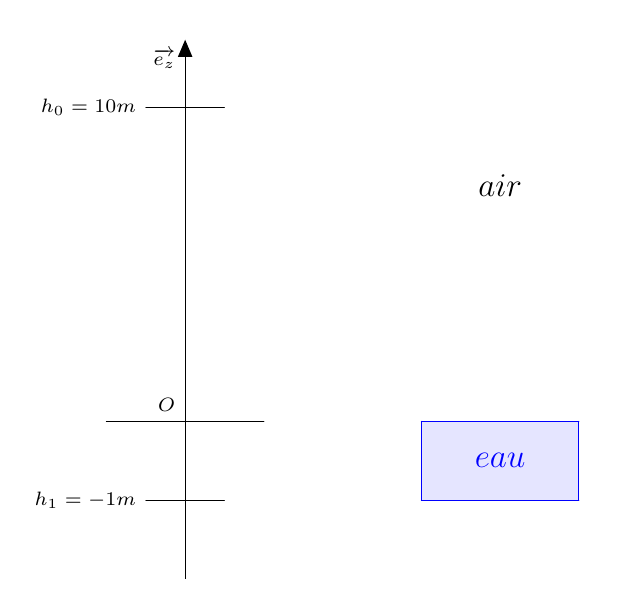
\begin{tikzpicture}[line cap=round,line join=round,>=triangle 45,x=1.0cm,y=1.0cm]
            \clip(0.,1.) rectangle (7.2,8.);
            \fill[line width=0.4pt,color=qqqqff,fill=qqqqff,fill opacity=0.10000000149011612] (5.,3.) -- (5.,2.) -- (7.,2.) -- (7.,3.) -- cycle;
            \draw [line width=0.4pt] (1.,3.)-- (3.,3.);
            \draw [->,line width=0.4pt] (2.,1.) -- (2.,7.846827418527504) node[font=\scriptsize, anchor = north east] {$\vec{e_{z}}$};
            \draw [line width=0.4pt] (1.50036389959032,6.991657966323216) node[font=\scriptsize, anchor = east] {$h_{0}
        = 10m$}-- (2.4971588856213867,6.991657966323216);
            \draw [line width=0.4pt] (1.50036389959032,2.) node[font=\scriptsize, anchor = east] {$h_{1} = -1 m$}-- (2.4971588856213867,2.);
            \draw (2, 3) node[font=\scriptsize,anchor = south east] {$O$};
            \draw [line width=0.4pt,color=qqqqff] (5.,3.)-- (5.,2.);
            \draw [line width=0.4pt,color=qqqqff] (5.,2.)-- (7.,2.);
            \draw [line width=0.4pt,color=qqqqff] (7.,2.)-- (7.,3.);
            \draw [line width=0.4pt,color=qqqqff] (7.,3.)-- (5.,3.);
            \begin{scriptsize}
            \draw[color=qqqqff] (6,2.5) node {$eau$};
            \draw[color=black] (6,6) node {$air$};
            \end{scriptsize}
            \end{tikzpicture}
        }
    \end{minipage}
    \begin{minipage}{.49\linewidth}
        \setlength{\parskip}{.3em}

        \begin{description}
            \item[Dans l'air:] $$p(0) - p(h_{0}) = \rho_{\text{air}} \cdot g \cdot (h_{0} - 0), \quad (h_{0} > 0)$$
            \item[Dansl l'eau:] $$p(h_{1}) - p(0) = \rho_{\text{eau}} \cdot g
                \cdot (0 - h_{1}), \quad (h_{1} < 0)$$
        \end{description}
    \end{minipage}
\end{center}

Ainsi, 

\begin{itemize}
    \item $p(0) = p(h_{0}) + \rho_{\text{air}} \cdot g \cdot h_{0} = (1.013
        \cdot 10^{5} + 1.3 \cdot 9.81 \cdot 10)Pa = 1.014 \cdot 10 ^{5} Pa$
    \item $p(h_{1}) = p(0) + \rho_{\text{eau}} g \cdot (-h_{1}) = (1.014 \cdot
        10^{5} + 1.3 \cdot 9.81 \cdot 1)Pa = 1.112 \cdot 10^{5}Pa $
\end{itemize}

\paragraph{Remarques:}

\begin{itemize}
    \item La vibration de pression de l'air peu souvent être négligée
    \item Pour $1m$ de profondeur dans l'eau, la pression augmente de $10\%$
\end{itemize}

\subsection{Surfaces connect\'e par un fluide}
\label{sub:surfaces_connect'e_par_un_fluide}

\begin{itemize}
    \item  La pression est identique en tous points d'un m\^eme niveau. Dans
        les vases communicants, les niveaux \`a l'air libre sont les m\^emes
        (sinon le fluide ne serait pas au repos)
    \item Soient deux colonnes de sections $S_{1}$ et $S_{2}$ reli\'ees par l'eau

        \begin{center}
            \begin{minipage}{.5\linewidth}
                \resizebox{\textwidth}{!}{
fig 1
                }
            \end{minipage}
            \begin{minipage}{.49\linewidth}
                \setlength{\parskip}{.3em}
                    Quelle force $\vec{F_{2}}$ faut-il exercer \`a droite pour
                    maintenir une diff\'erence de niveau $\Delta h = h_{1} -
                    h_{2}$ entre les colonnes d'eau?
            \end{minipage}
        \end{center}

    \item Au niveaux de $h_{2}$, la pression est la m\^eme dans les 2 colonnes
        $$\cancel{p_{a}} + \frac{F_{2}}{S_{2}} = \cancel{p_{a}} +
        \frac{M_{a}}{S_{1}}+\rho_{\text{eau}} g \cdot (h_{1} - h_{2}) \implies
        F_{2} = M\cdot g \cdot \frac{S_{2}}{S_{1}} + \rho_{\text{eau}} \cdot g
        \cdot (h_{2} - h_{1}) cdto S_{2} $$
    \item En choisissant $S_{2}$ petite, $F_{2}$ peut \^etre petite. C'est le
        principe de fonctionnement d'une propre hydraulique.
\end{itemize}

\subsection{Principe d'Archim\`ede}
\label{sub:principe_d_archim`ede}

La pression augmente avec la profondeur, donc un corps immerg\'e subit une
r\'esultante des forces de pression dirig\'ee vers le haut appel\'ee pouss\'ee
d'Archim\`ede $\vec{F_{A}}$.

\begin{center}
    \begin{minipage}{.5\linewidth}
        \resizebox{\textwidth}{!}{
fig2
        }
    \end{minipage}
    \begin{minipage}{.49\linewidth}
        \setlength{\parskip}{.3em}
        \begin{description}
            \item[Objet:] \'el\'ement de fluide de masse $m$ et de volume $V_{\text{fl}}$
            \item[Forces:] $m\cdot \vec g$ poids, forces de pression (pouss\'ee
                d'Arhcim\`ede)
                $$m \cdot \vec g + \vec{F_{A}}  = \vec 0 \implies \vec{F_{A}} =
                - \rho_{\text{fl}} \cdot V_{\text{fl}} \cdot \vec g$$
        \end{description}
    \end{minipage}
\end{center}

Le point d'application de la pouss\'ee d'Archim\`ede est le centre de masse de
l'\'el\'ement de fluide.

Si on remplace l'\'el\'ement de fluide par un autre corps au repos de m\^eme
forme et de m\^eme volume, les forces exerc\'ees par le fluide environnant ne
changent pas.

\paragraph{Pouss\'ee d'Archim\`ede:}
\label{par:pouss'ee_d_archim`ede_}

\begin{equation}
    \label{eq:3.40} %TODO check, on latex this equation is .38, during the lesson was .40
    \vec{F_{A}} = - \rho_{\text{fl}} \cdot V_{\text{im}} \cdot \vec g
\end{equation}
o\`u $V_{\text{im}}$ est le volume immerg\'e du corps.

\paragraph{Remarque:}

Comme la pouss\'ee d'Archim\`ede est une cons\'equence de la loi de l'hydrostatique 
qui donne la diff\'erence de pression dans un m\^eme fluide, un corps flottant
entre deux fluides subit deux pouss\'ees d'Archim\`ede, selon le volume
immerg\'e dans chacun des fluides.


\paragraph{Exemple:}

Un ballon sur l'eau se trouve partiellement dans l'eau et partiellement dans
l'air.

\subsection{Applications de la force d'Archim\`ede}
\label{sub:applications_de_la_force_d_archi}

\begin{enumerate}
    \item Ballon de foire retenu au sol par un fil.

        \begin{center}
            \begin{minipage}{.4\linewidth}
                \resizebox{\textwidth}{!}{
fig 3
                }
            \end{minipage}
            \begin{minipage}{.59\linewidth}
                \setlength{\parskip}{.3em}
                \begin{description}
                    \item[Objet:] ballon
                    \item[Forces:] poids $m \cdot \vec g$, tension $\vec T$,
                        pouss\'ee d'Archim\`ede $\vec{F_{A}}$
                        $$m \cdot \vec g + \vec T+ \vec{F_{A}} = \vec O$$
                        \begin{equation}
                            \label{eq:3.41}
                            \vec T = - m\cdot \vec g- \vec{F_{A}} = (\rho_{\text{air}}\cdot
                            V - m) \cdot \vec g
                        \end{equation}
                        \item Le fil est vertical et tendu si $\rho_{\text{air}}
                        \cdot V -m > 0$
                \end{description}
            \end{minipage}
        \end{center}

    \item Fluide qui se trouve dans un chariot acc\'el\'er\'e

        \begin{center}
            \begin{minipage}{.5\linewidth}
                \resizebox{\textwidth}{!}{
fig 4
                }
            \end{minipage}
            \begin{minipage}{.49\linewidth}
                \setlength{\parskip}{.3em}
                \begin{description}
                    \item[Objet:] \'el\'ement de fluide 
                    \item[Forces:] poids $m\cdot \vec g$, forces de pression (pouss\'ee
                        d'Archim\`ede $\vec{F_{A}}$)
                        \begin{equation}
                            m \cdot \vec g + \vec{F_{A}} = m\cdot \vec a 
                        \end{equation}
                        $$\implies \vec{F_{A}} = - \underbrace{\rho_{\text{fl}} \cdot V_{\text{im}}}_{=m}
                        \cdot (\vec g - \vec a)$$

                    \Warning $\vec{F_{A}}$ n'est pas verticale (hydrodynamique
                    si $\vec a \neq \vec 0$)

                \end{description}
            \end{minipage}
        \end{center}

    \item Ballon de foire au plancher d'un chariot acc\'el\'er\'e

        \begin{center}
            \begin{minipage}{.5\linewidth}
                \resizebox{\textwidth}{!}{
fig 5
                }
            \end{minipage}
            \begin{minipage}{.49\linewidth}
                \setlength{\parskip}{.3em}

                \begin{description}
                    \item[Objet:] ballon
                    \item[Forces:] poids $m \cdot \vec g$, tension du fil $\vec T$,
                        pouss\'ee d'Archim\`ede
                        \begin{equation}
                            m\cdot \vec g + \vec{F_{A}}+ \vec T= m \cdot \vec a
                        \end{equation}
                        $$\implies \vec T = - m \cdot (\vec g - \vec a) - \vec{F_{A}}
                        = (\rho_{\text{air}}\cdot V - m) \cdot (\vec g - \vec a)$$
                \end{description}
            \end{minipage}
        \end{center}
        Le fil est tendu si et seulement si $\rho_{\text{air}} \cdot V - \underbrace{m}_{\rho_{\text{gaz}} \cdot V} > 0$
        et l'angle est donn\'e par:
        $$\tan(\alpha) = \frac{T_{x}}{T_{y}} = \frac{- (\rho_{\text{air}} \cdot V - m) \cdot a}{-
        (\rho_{\text{air}} \cdot V - m) \cdot g} = \frac{a}{g}$$
        $$\alpha = \arctan(\frac{a}{g})$$
\end{enumerate}

\subsection{Unit\'e de pression: le $mmHg$ }
\label{sub:unit'e_de_pression_le_mmhg_}

La pression atmosph\'erique peut \^etre donn\'ee par la hauteur d'une colonne de
liquide dans un tube.

\begin{center}
    \begin{minipage}{.5\linewidth}
        \resizebox{\textwidth}{!}{
fig 6
        }
    \end{minipage}
    \begin{minipage}{.49\linewidth}
        \setlength{\parskip}{.3em}
        \begin{itemize}
            \item Un tube vide, ferm\'e sup\'erieurement, plong dans du mercure
                ($Hg$). Sans l'effet de la pression ambiante $p_{a}$, le mercure
                monte dans le tube.
            \item La pression $p_{a}$ est partout la m\^eme au niveau de
                l'interface air-mercure.
        \end{itemize}
    \end{minipage}
\end{center}

Sous la colonne de mercure,
\begin{equation}
    p_{Hg} = p_{a} = \rho_{Hg} \cdot g \cdot h \iff h = \frac{p_{a}}{\rho_{Hg} \cdot g}
\end{equation}

A une atmosph\`ere, la hauteur de la colonne est de $760 mm$, on a la relation, 
\begin{equation}
    \frac{h}{760mm} = \frac{p_{a}}{1 atm}
\end{equation}


 28/03/2019

\section{Deux intermèdes}
\label{sec:deux_intermedes}

\subsection{Produit scalaire}
\label{sub:produit_scalaire}

Soient deux vecteurs $\vec a$ et $\vec b$. Leur produit scalaire s'écrit:

\begin{center}
    \begin{minipage}{.5\linewidth}
        \resizebox{\textwidth}{!}{
fig 1
        }
    \end{minipage}
    \begin{minipage}{.49\linewidth}
        \setlength{\parskip}{.3em}
        \begin{equation}
            \label{eq:3.46}
            \vec a \cdot \vec b = \| \vec a \| \cdot \|\vec b\| \cdot \cos(\phi)
        \end{equation}
        où $\phi$ est l'angle formé par $\vec a$ et $\vec b$.
    \end{minipage}
\end{center}

Le produit scalaire est une mesure du parallélisme de deux vecteurs.

\paragraph{Propriétés:}

\begin{itemize}
    \item $\vec a \cdot \vec b = \vec b \cdot \vec a$
    \item Si l'angle est aigu: $\phi \in \left[-\frac{\pi}{2};\frac{\pi}{2} \right]
        \iff \vec a \cdot \vec b > 0$
    \item si l'angle est obtus: $\phi \in \left]\frac{\pi}{2};\frac{3\pi}{2} \right]
        \iff \vec a \cdot \vec b < 0$
    \item Si $\vec a$ et $\vec b$ sont orthogonaux: $\phi \in \left\{-\frac{\pi }{2}; \frac{\pi }{2}\right\} \iff
        \vec a \cdot \vec b = 0$
    \item Si $\vec a \equiv \vec b \implies \| \vec b \| = \| \vec a \|$
        et $\cos(\phi) = \cos(0) = 1 \implies \vec a \cdot \vec a = \|\vec{a} \|
        ^{2}$
\end{itemize}

\paragraph{Cas particuliers}
\label{par:cas_particuliers}

$$\| \vec b \| = 1 \implies \vec a \cdot \vec b = \| \vec a\| \cdot \cos(\phi)$$
est la projection (avec signe) du vecteur $\vec a$ le long du vecteur unitaire $\vec b$.
On peut ainsi obtenir les composantes d'un vecteur $\vec a$ dans un repère
orthonormée $(O, \vec{e_{x}}, \vec{e_{y}})$ par produit scalaire: 
$$a_{x} = \vec a \cdot \vec{e_{x}} $$
$$a_{y} = \vec a \cdot \vec{e_{y}} $$

\subsection{Dérivée temporelle d'un produit}

La dérivé temporelle d'un produit (algébrique, scalaire, vectoriel) se calcule
come suit:

\[
    \begin{split}
        \frac{d}{dt} (AB) &= \lim_{\Delta t \to 0} \frac{\Delta (AB)}{\Delta t}
        = \lim_{\Delta t \to 0} \frac{1}{\Delta t} \left[A(t + \Delta t) \cdot
            B(t + \Delta t) - A(t) \cdot B(t)\right]\\
        \Delta (AB) &= A(t + \Delta t) \cdot B(t + \Delta t) - A(t) \cdot B(t +
        \Delta t) + A(t) \cdot B(t + \Delta t) - A(t) \cdot B(t) \\
        &=(A(t + \Delta t) - A(t)) \cdot B(t+\Delta t) + A(t) \cdot (B(t + \Delta t) - B(t))\\
        &= \Delta A \cdot B(t + \Delta t) + A(t) \cdot \Delta B\\
        \frac{d}{dt}(AB) &= \lim_{\Delta t \to 0} \frac{\Delta (AB)}{\Delta t} =
        \lim_{\Delta t \to 0} \frac{\Delta A}{\Delta t} \cdot \overbrace{B(t + \Delta t)}^{\to
        B(t)} + \lim_{\Delta t \to 0} A(t) \cdot \frac{\Delta B}{\Delta t} t) - B(t))\\
    \end{split}
\]

\begin{equation}
    \label{eq:3.47}
    \frac{d}{dt} (AB) = \dot A B + A \dot B 
\end{equation}

Pour un vecteur $\vec v = v \cdot \vec{e_{t}}$

\begin{equation}
    \label{eq:3.48}
    \frac{d}{dt} \vec v = \frac{d}{dt}(v \cdot \vec{e_{t}}) = \dot v \cdot \vec{e_{t}}
    + v\cdot \dot{\vec{e_{t}}}
\end{equation}

\paragraph{Remarque:}

Le premier terme $\dot v \cdot \vec{e_{t}}$ correspond à la dérivée du vecteur $\vec v$
lorsque sa norme varie et son orientation reste constante. Le deuxième $v \cdot
\dot{\vec{e_{t}}}$ correspond à la dérivée du vecteur $\vec v$ lorsque son
orientation varie mais sa norme $v$ reste constante.

Pour le carré de la norme du vecteur $\vec v$ :

\begin{equation}
    \label{eq:3.49}
    \frac{d}{dt} v^{2}  = \frac{d}{dt} (\vec v \cdot \vec v) = \dot{\vec v} \cdot
    \vec v + \vec v \cdot \dot{\vec v} = 2 \cdot \vec v \cdot \dot{\vec v}
\end{equation}

\paragraph{Remarque:}
Lorsque le norme du vecteur $\vec v$ est constante et $\dot{\vec v} \neq 0$, le
vecteur $\vec v$ est orthohonale à sa dérivée temporelle $\dot{\vec v}$,
c'est-à-dire que $\vec v \cdot \dot{\vec v}=0$ 


\section{Repère lié au mouvement}

\subsection{Abscisse curviligne, repère}

\paragraph{Rappel:}
\label{par:rappel_}

Dans le plan muni d'un repère orthonormé $(O, \vec{e_{x}}, \vec{e_{y}})$

\begin{center}
    \begin{minipage}{.5\linewidth}
        \resizebox{\textwidth}{!}{
 fig 2
        }
    \end{minipage}
    \begin{minipage}{.49\linewidth}
        \setlength{\parskip}{.3em}
        \begin{itemize}
            \item $x$ est la coordonnée d'abscisse et $\vec{e_{x}}$ donne le
                sens positif:
            \item $x > 0 : P$ est devant $O$ selon $\vec{e_{x}}$
            \item $x < 0: Q$ est derrière $O$ selon $\vec{e_{x}}$
        \end{itemize}
    \end{minipage}
\end{center}


\paragraph{Généralisation à une courbe $\Gamma$ du plan:}
\label{par:generalisation_a_une_courbe_gamma_du_plan}


On prend un point $O$ sur $\Gamma$ comme origine et on choisit un sens positif
de parcours. La position d'un objet sur $\Gamma$ est donné par la longueur $s$
(avec signe) mesurée le long de $\Gamma$.


\paragraph{Abscisse curviligne}
\label{par:abscisse_curviligne}


\begin{center}
    \begin{minipage}{.5\linewidth}
        \resizebox{\textwidth}{!}{
 fig 3
        }
    \end{minipage}
    \begin{minipage}{.49\linewidth}
        \setlength{\parskip}{.3em}
        \begin{itemize}
            \item $s$ est l'abscisse curviligne 
            \item $s > 0: P$ est devant $O$ selon $\vec{e_{t}}$
            \item $s < 0: Q$ est derrière $O$ selon $\vec{e_{t}}$
        \end{itemize}
    \end{minipage}
\end{center}

On définit un repère orthonormé mobile lié au point matériel $P (P, \vec{e_{t}},
\vec{e_{n}})$ qui se déplace avec $P$ le long de $\Gamma$.

\begin{enumerate}
    \item $\vec{e_{t}}$ est un vecteur normé, tangent à la trajectoire $\Gamma$
        et donnant le sens positif du parcours
    \item $\vec{e_{n}}$ un vecteur normé, normal à $\Gamma$ et formant en $P$ un
        angle $\frac{\pi}{2}$ avec $\vec{e_{t}}$ (orienté vers l'intérieur)
\end{enumerate}

\paragraph{Exemple:}

\begin{center}
    \begin{minipage}{.44\linewidth}
        \resizebox{\textwidth}{!}{
fig 4
        }
    \end{minipage}
    \begin{minipage}{.55\linewidth}
        \setlength{\parskip}{.3em}
        \begin{description}
            \item[Abscisse curviligne:] $s = L \cdot \alpha$ où $\alpha \in
                \left[- \frac{\pi }{2}; \frac{\pi }{2}\right]$
            \item  $\alpha > 0:$ gauche
            \item  $\alpha < 0:$ droite
        \end{description}
    \end{minipage}
\end{center}

\subsection{Vitesse scalaire}
\label{sub:vitesse_scalaire}

En tout point de la trajectoire $\Gamma$ d'un objet, la vitesse est toujours
tangente  à la trajectoire s'écrit,
$$\vec v = v \cdot \vec{e_{t}}$$

où $v$ est la composante scalaire de la vitesse le long de la trajectoire $\Gamma$
et $\vec{e_{t}}$ est le vecteur unitaire tangent.

\begin{itemize}
    \item La vitesse scalaire est définie comme la dérivée temporelle de
        l'abscisse curviligne:
        \begin{equation}
            \label{eq:3.50}
            v = \lim_{\Delta t \to 0} \frac{\Delta s}{\Delta t} = \dot s
        \end{equation}
    \item Unité physique (SI): $\left[\frac{m}{s}\right]$
\end{itemize}

\paragraph{Remarque:}

$\| \vec v \| = v$  (vitesse instantanée)
\paragraph{Exemple:}

Trajet Lausanne-Evian:

\begin{itemize}
    \item Vitesse moyenne:
        $$\|\vec{V_{\text{moy}}}\| = \|\frac{\Delta \vec v}{\Delta t}\| - \frac{15
        km}{1.5 h} = 10 \frac{km}{h}$$

    \item Vitesse scalaire moyenne:
        $$V_{\text{moy}} = \frac{\Delta s}{\Delta t} = \frac{120 km}{1.5h} = 80
        \frac{km}{h}$$
        $$\implies \| \vec{v_{\text{moy}}}\| \neq V_{\text{moy}} \Warning$$
\end{itemize}


\subsection{Accélération tangentielle et normale}

En tout point $P$ de la trajectoire $\Gamma$ d'un objet, l'accélération se
décompose dans un repère $(P, \vec{e_{t}}, \vec{e_{n}})$ comme suit:

\begin{center}
    \begin{minipage}{.5\linewidth}
        \resizebox{\textwidth}{!}{
 fig 5
        }
    \end{minipage}
    \begin{minipage}{.49\linewidth}
        \setlength{\parskip}{.3em}
        \begin{description}
            \item[Accélération:]  
                \begin{equation}
                    \label{eq:3.51}
                    \vec a = \vec{a_{t}} + \vec{a_{n}}
                \end{equation}
            \item[Accélération tangentielle:] 
                $$\vec{a_{t}} = a_{t} \cdot \vec{e_{t}} = (\vec a \cdot \vec{e_{t}})
                \cdot \vec{e_{t}} \text{ où } \|\vec{e_{t}}\| = 1$$

            \item[Accélération normale:] 
                $$\vec{a_{n}} = a_{n} \cdot \vec{e_{n}} = (\vec a \cdot \vec{e_{n}})
                \cdot \vec{e_{n}} \text{ où } \|\vec{e_{n}}\| = 1$$
        \end{description}
    \end{minipage}
\end{center}

\begin{enumerate}
    \item L'accélération tangentielle scalaire est l'accélération le long de la
        trajectoire et donc la dérivée temporelle de la vitesse scalaire.
        \begin{equation}
            \label{eq:3.52}
            a_{t} = \lim_{\Delta t \to 0} \frac{\Delta v}{\Delta t} = 
            \dot v = \ddot s 
        \end{equation}

        Unité physique (SI): $\left[\frac{m}{s^{2}}\right]$
        \begin{itemize}
            \item $a_{t} > 0: v$ augmente (l'objet va plus vite dans le sens $\vec{e_{t}}$)
            \item $a_{t} < 0: v$ diminue (l'objet va plus lentement dans le sens $\vec{e_{t}}$)
        \end{itemize}

    \item L'accélération normale scalaire est la dérivée temporelle de la
        direction de la vitesse $\vec v$

        \begin{equation}
            \label{eq:3.53}
            a_{n} = \frac{v^{2}}{R}
        \end{equation}
        où $R$ est le rayon de courbure de la trajectoire à un instant donné
        (rayon du cercle osculateur passant par trois points infiniment proches
        de la trajectoire).

        Unité physique (SI): $\left[\frac{m}{s^{2}}\right]$

        L'accélération normale est toujours orientée vers l'intérieur de la
        trajectoire.

        \paragraph{Remarque:}
        
        Les relations $\eqref{eq:3.52}$ et $\eqref{eq:3.53}$ sont une
        conséquence des intermèdes 3.9, comme on va le montrer.

        En effet, l'accélération s'écrit comme,
        $$\vec a = \dot{\vec v} = \frac{d}{dt} (v \cdot \vec{e_{t}}) = \dot v
        \cdot \vec{e_{t}} + v \cdot \dot{\vec{e_{t}}}$$

        Comme  $\| \vec{e_{t}}\|^{2} = 1; \frac{d}{dt} \|\vec{e_{t}}\|^{2} =
        \frac{d}{dt} (\vec{e_{t}} \cdot \vec{e_{t}}) = \dot{\vec{e_{t}}} \cdot
        \vec{e_{t}} + \vec{e_{t}}\cdot \dot{\vec{e_{t}}} = 2 \cdot \vec{e_{t}}
        \cdot \dot{\vec{e_{t}}} = 0$
        La dérivée temporelle $\dot{\vec{e_{t}}}$ est donc soit nulle, soit
        normale à $\vec{e_{t}}$. Ainsi $\vec{a_{t}} = \dot v \cdot \vec{e_{t}}$
        et $\vec{a_{n}} = v \cdot \dot{\vec{e_{t}}}$


\end{enumerate}

\end{document}
